\newpage
\section{Colective exploration algorithms type I \& II analysis}

Several test have been done by means of $\rho$ and $k$ combinations taken values in the next sets: $$\rho = \{0.01, 0.5\}, k = \{5, 10, 15, 50, 100\}$$

\subsection{Set $\rho = 0.1, k=5$}

\begin{figure}[ht]
\centering
\subfigure[Fitness evolution]{
	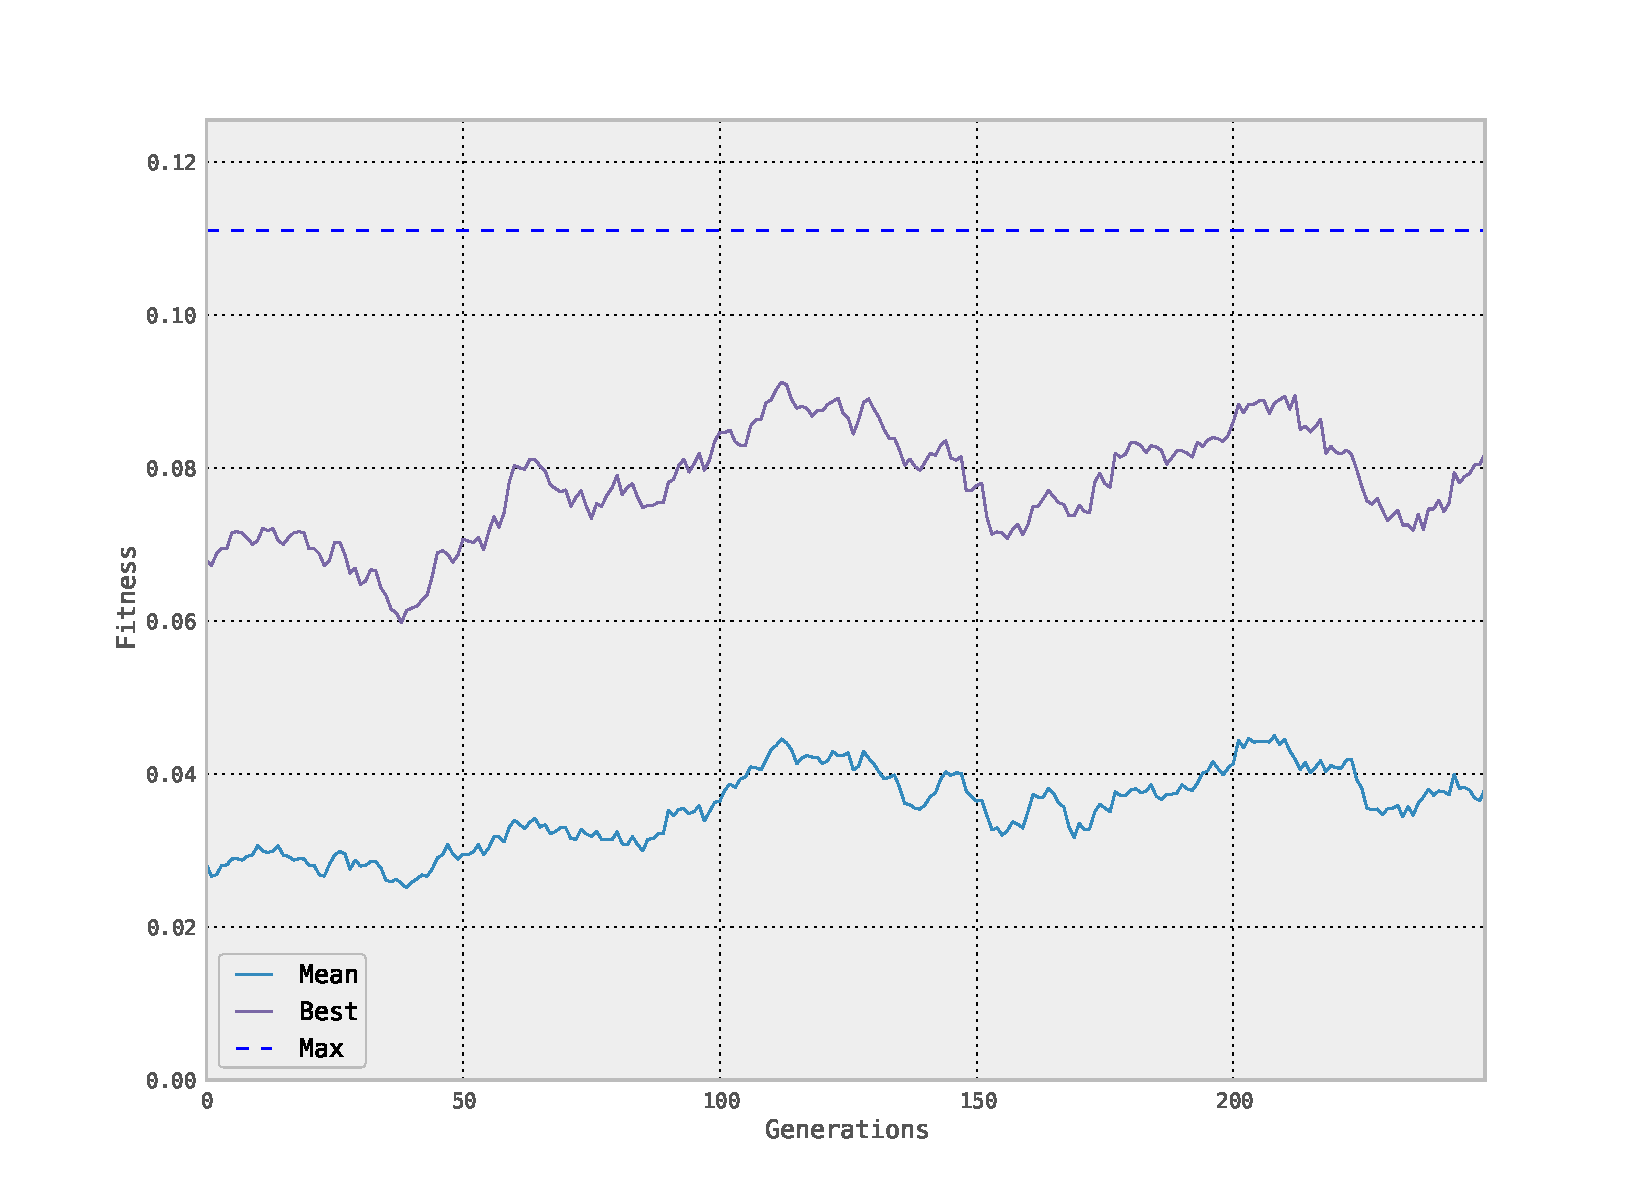
\includegraphics[scale =0.4] {images/section3/fitness_1_5_001.pdf}
	\label{fig:subfig11}
}
\subfigure[Pheromones per edge]{
	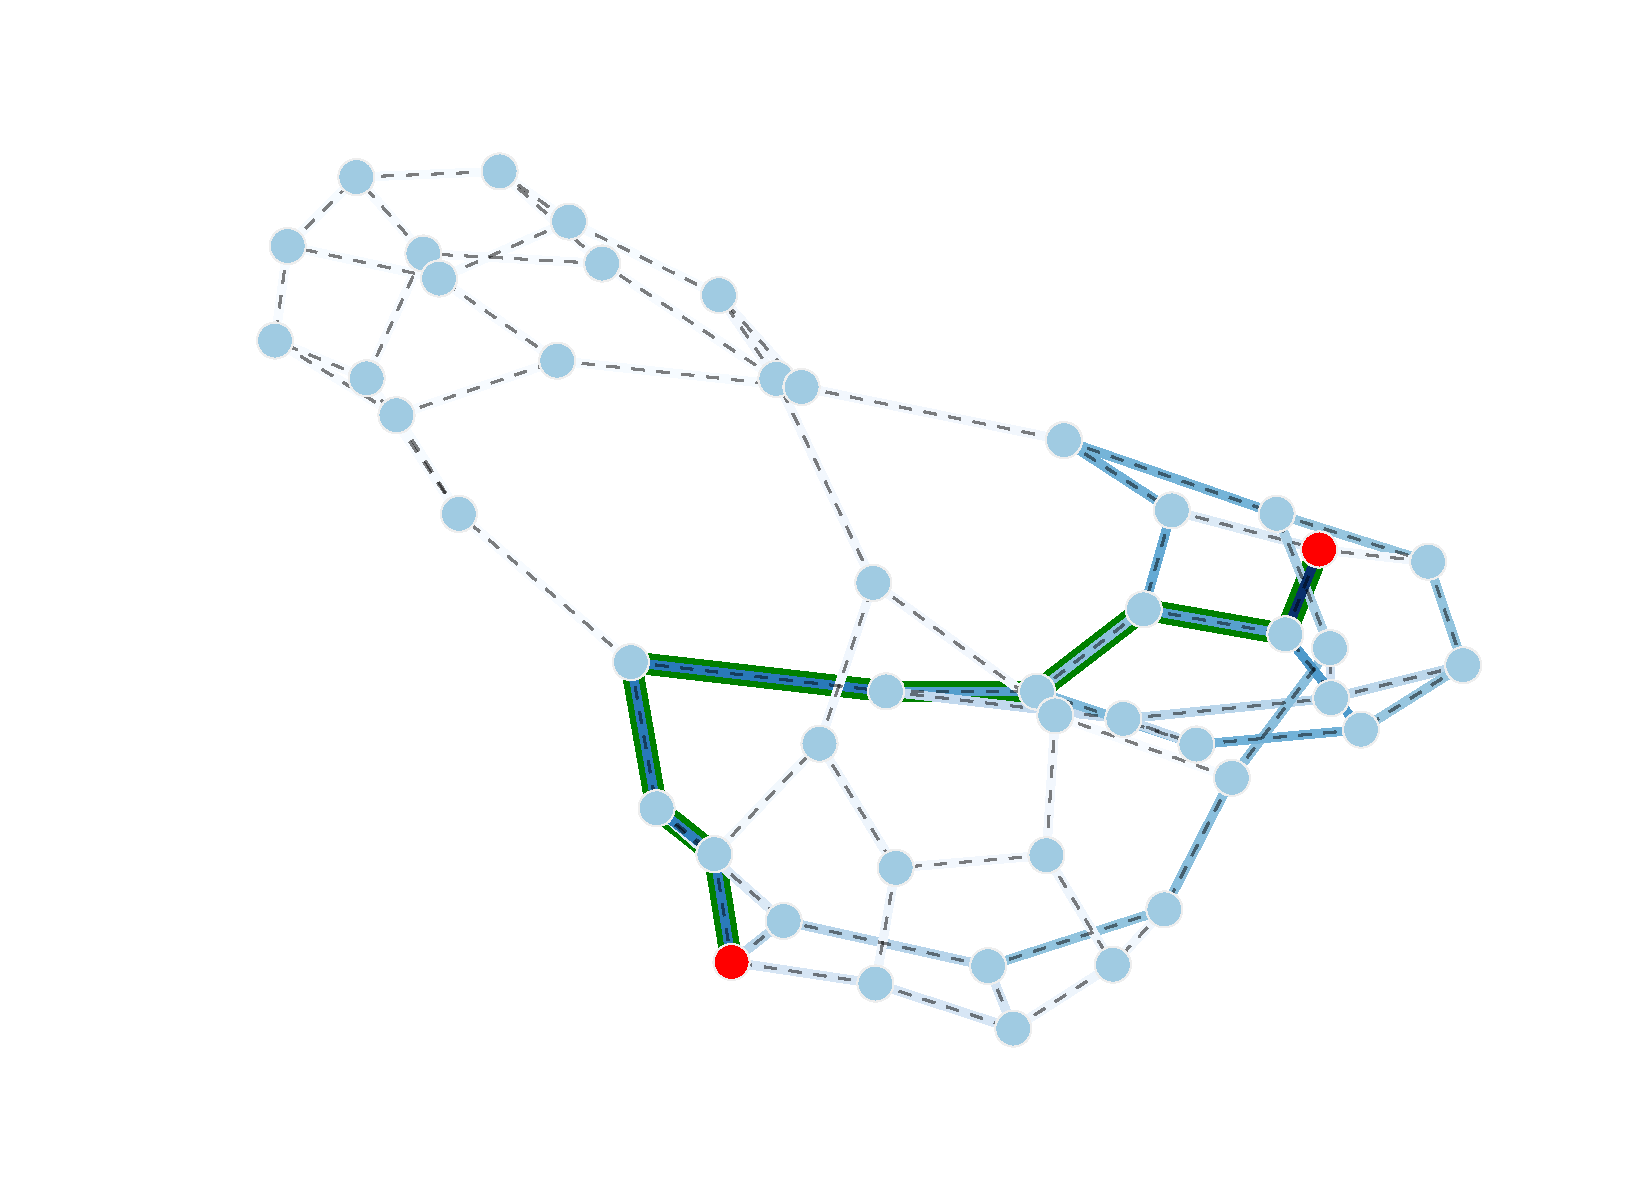
\includegraphics[scale =0.4] {images/section3/pheromones_5_001.pdf}
	\label{fig:subfig12}
}
%\caption[Optional caption for list of figures]{Caption of subfigures \subref{fig:subfig1}, \subref{fig:subfig2}}
\label{fig:fig1}
\end{figure}


\newpage
\subsection{Set $\rho = 0.1, k=10$}

\begin{figure}[ht]
\centering
\subfigure[Fitness evolution]{
	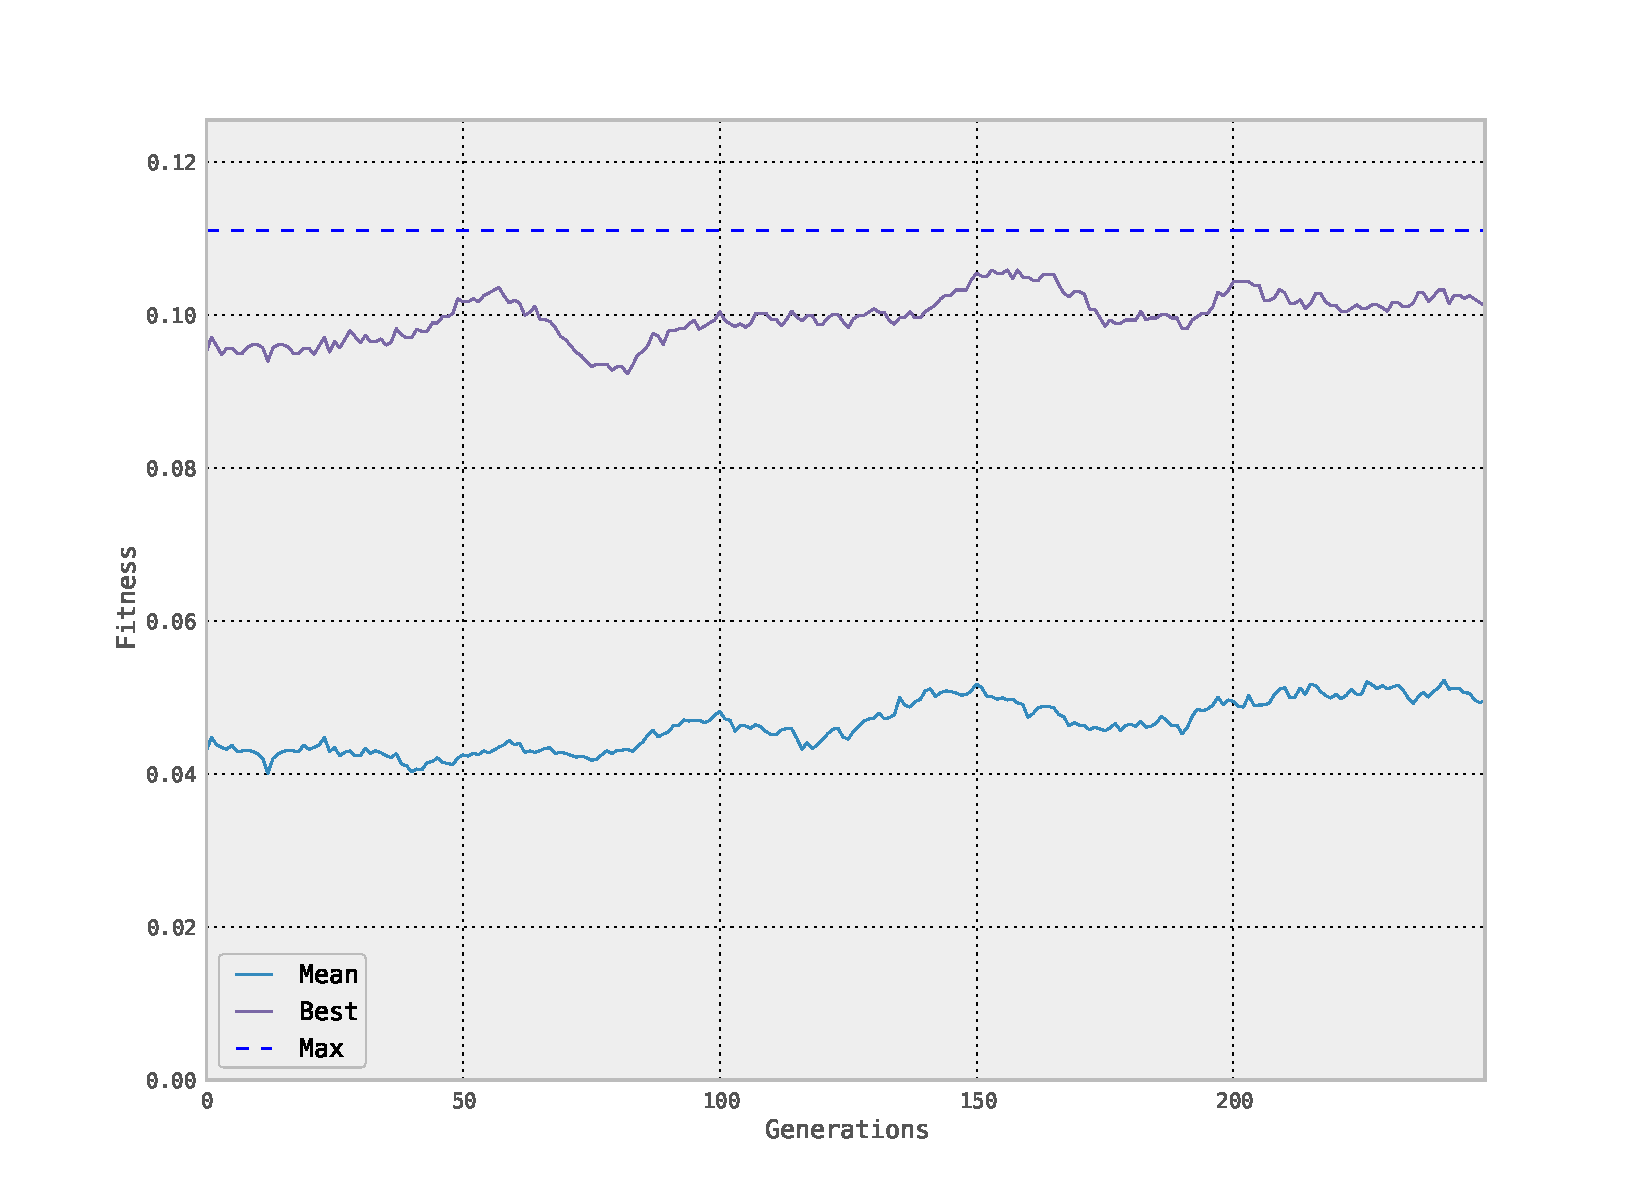
\includegraphics[scale =0.4] {images/section3/fitness_1_10_001.pdf}
	\label{fig:figure23}
}
\subfigure[Pheromones per edge]{
	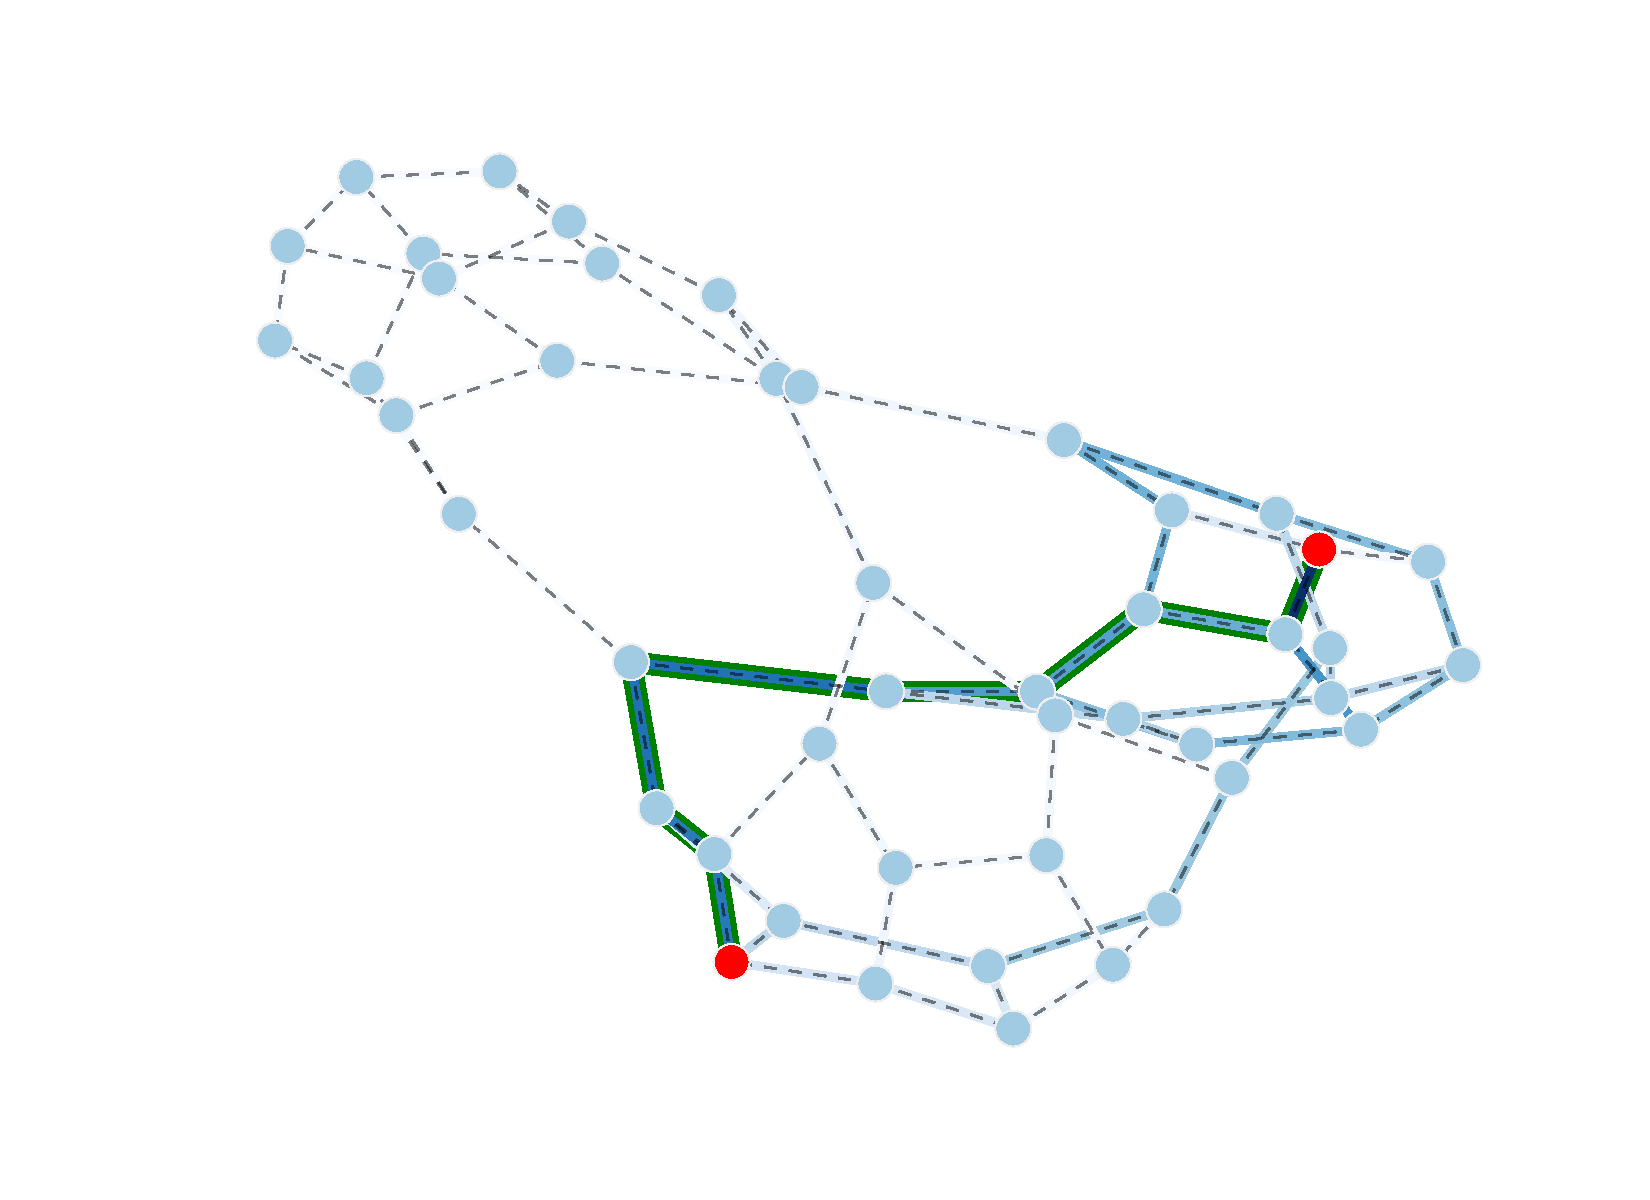
\includegraphics[scale =0.4] {images/section3/pheromones_10_001.pdf}
	\label{fig:figure22}
}
%\caption[Optional caption for list of figures]{Caption of subfigures \subref{fig:subfig1}, \subref{fig:subfig2}}
\label{fig:figure2}
\end{figure}





\newpage
\subsection{Set $\rho = 0.1, k=15$}

\begin{figure}[ht]
\centering
\subfigure[Fitness evolution]{
	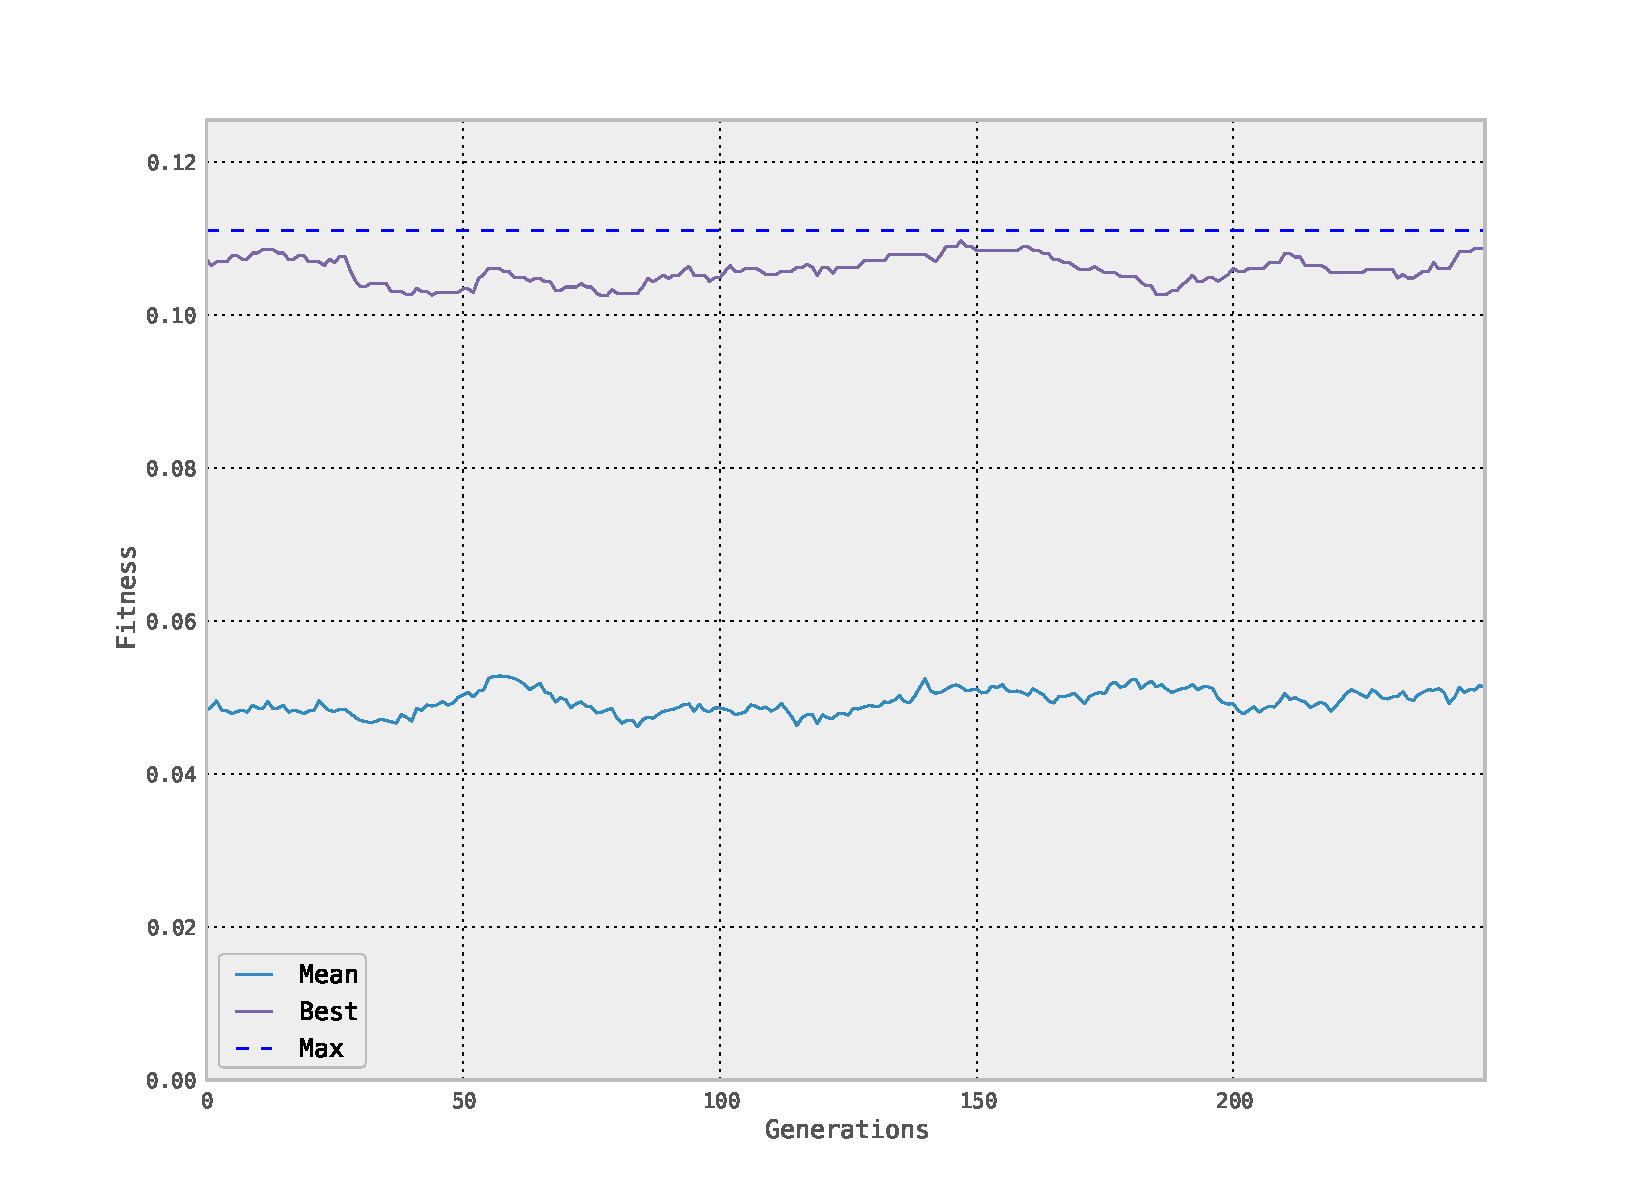
\includegraphics[scale =0.4] {images/section3/fitness_1_15_001.pdf}
	\label{fig:figure31}
}
\subfigure[Pheromones per edge]{
	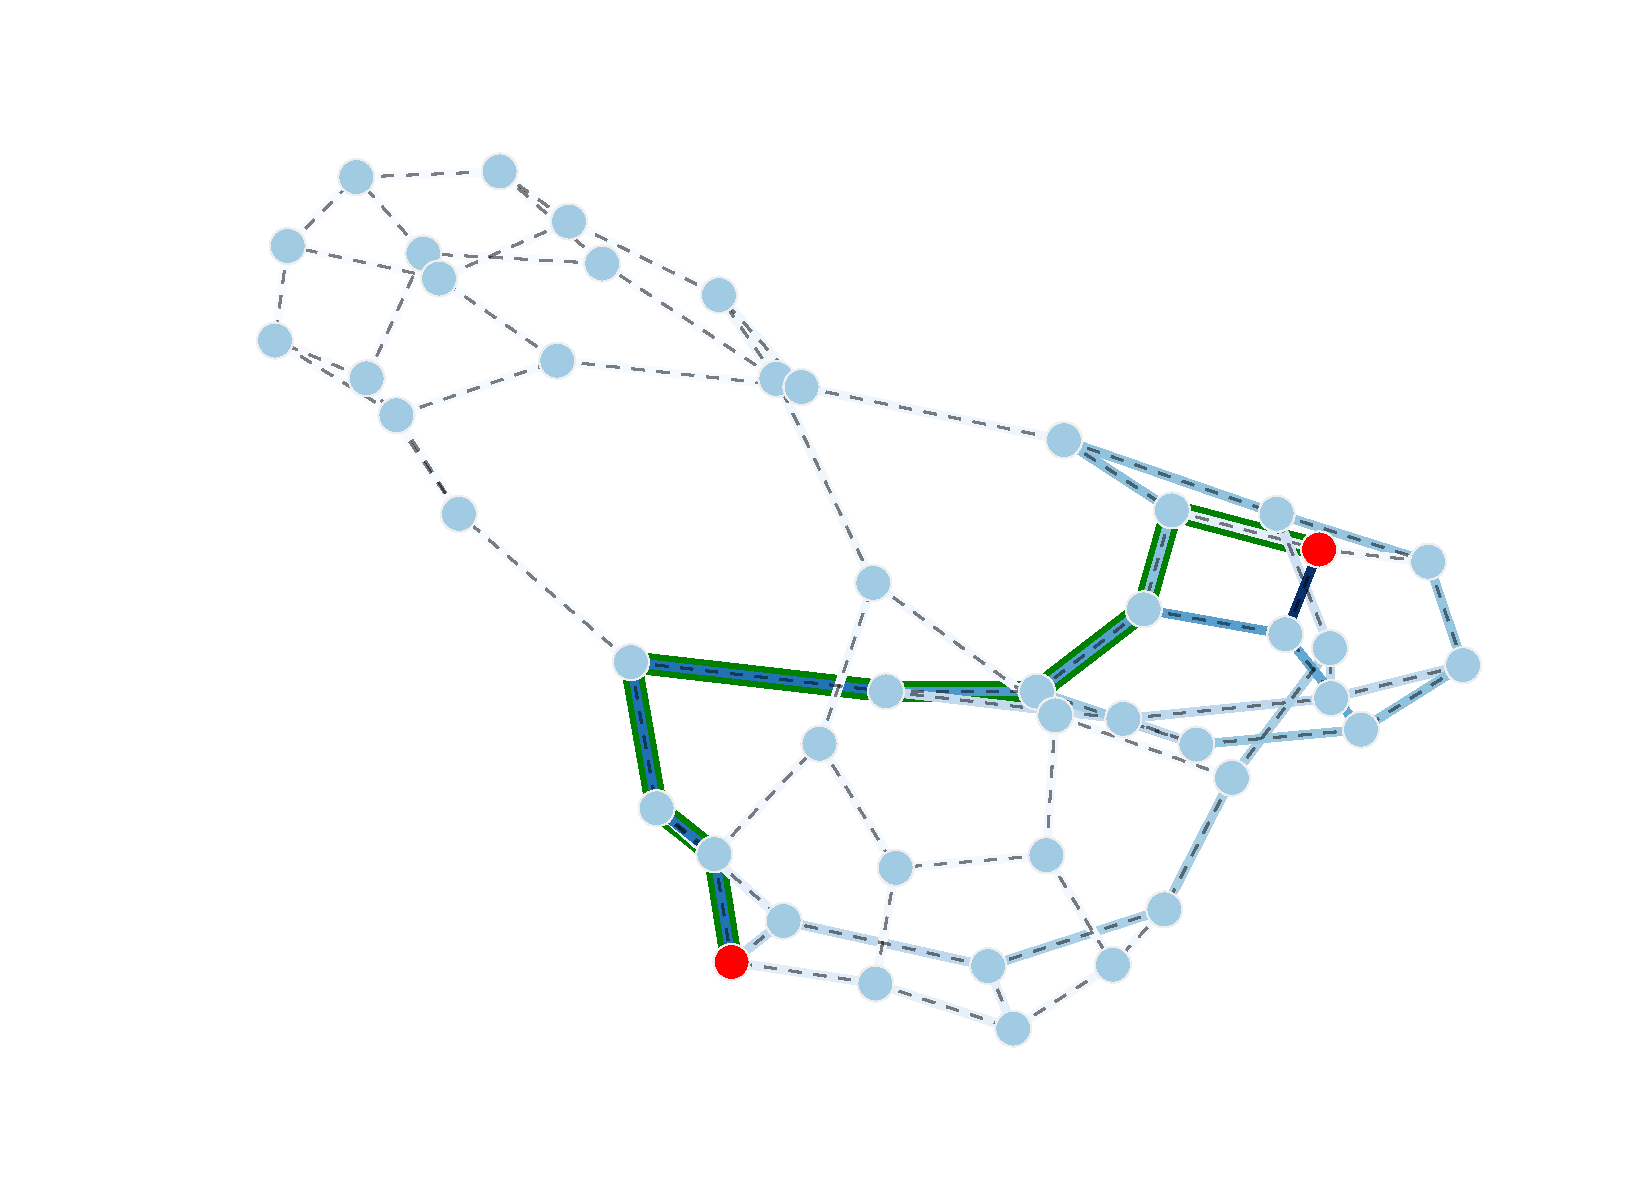
\includegraphics[scale =0.4] {images/section3/pheromones_15_001.pdf}
	\label{fig:figure32}
}
%\caption[Optional caption for list of figures]{Caption of subfigures \subref{fig:subfig1}, \subref{fig:subfig2}}
\label{fig:figure3}
\end{figure}


\newpage
\subsection{Set $\rho = 0.1, k=50$}

\begin{figure}[ht]
\centering
\subfigure[Fitness evolution]{
	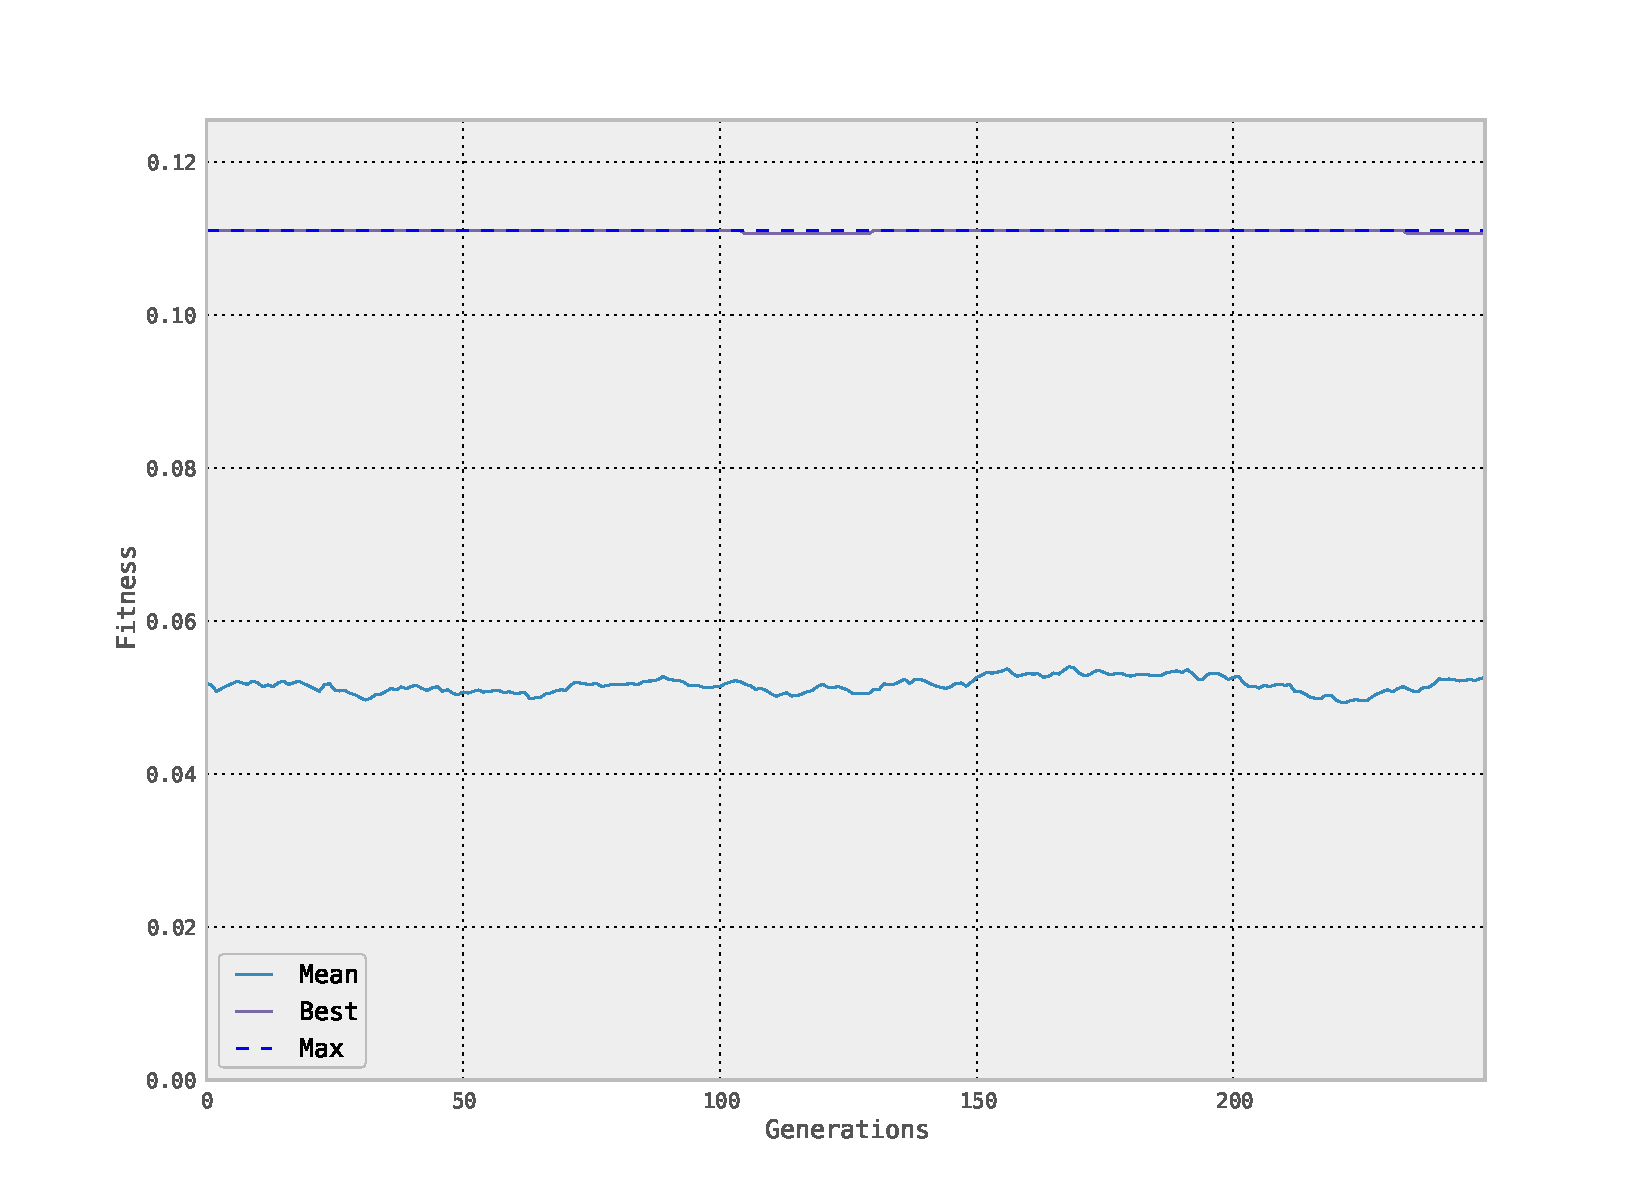
\includegraphics[scale =0.4] {images/section3/fitness_1_50_001.pdf}
	\label{fig:figure41}
}
\subfigure[Pheromones per edge]{
	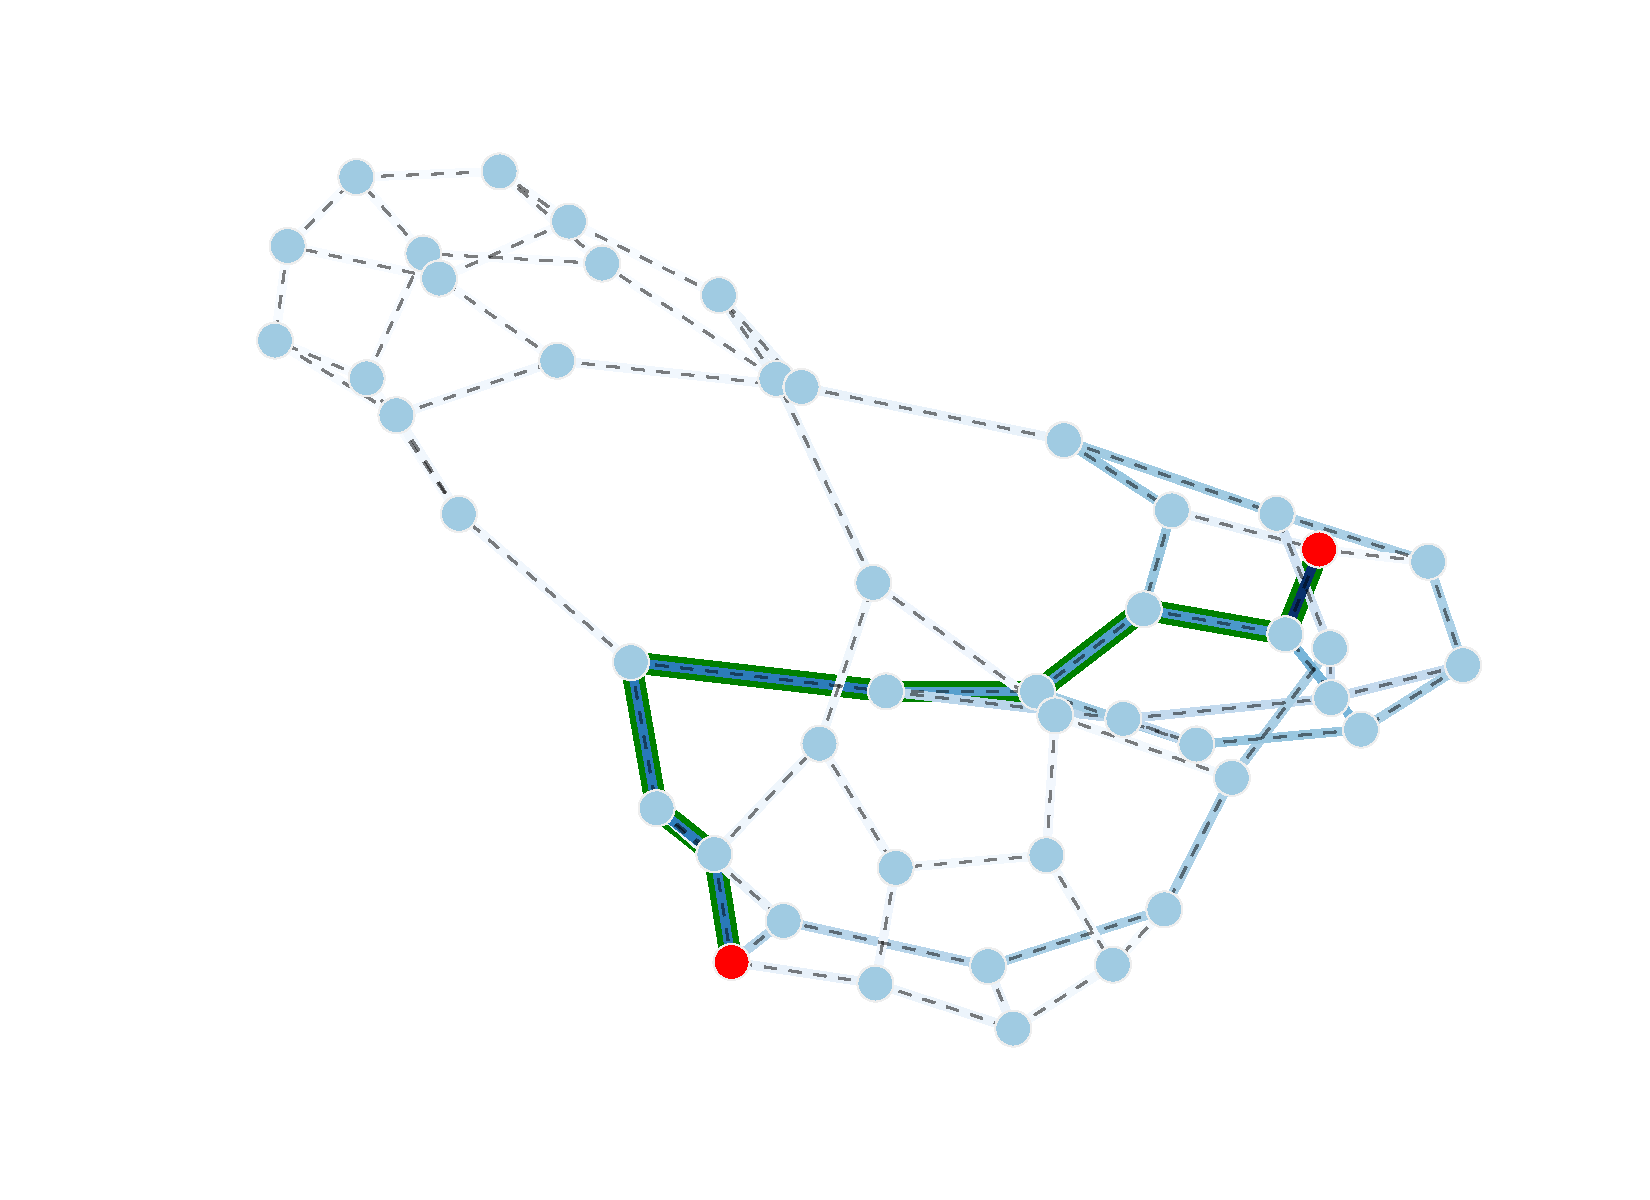
\includegraphics[scale =0.4] {images/section3/pheromones_50_001.pdf}
	\label{fig:figure42}
}
%\caption[Optional caption for list of figures]{Caption of subfigures \subref{fig:subfig1}, \subref{fig:subfig2}}
\label{fig:figure4}
\end{figure}




\newpage
\subsection{Set $\rho = 0.1, k=100$}

\begin{figure}[ht]
\centering
\subfigure[Fitness evolution]{
	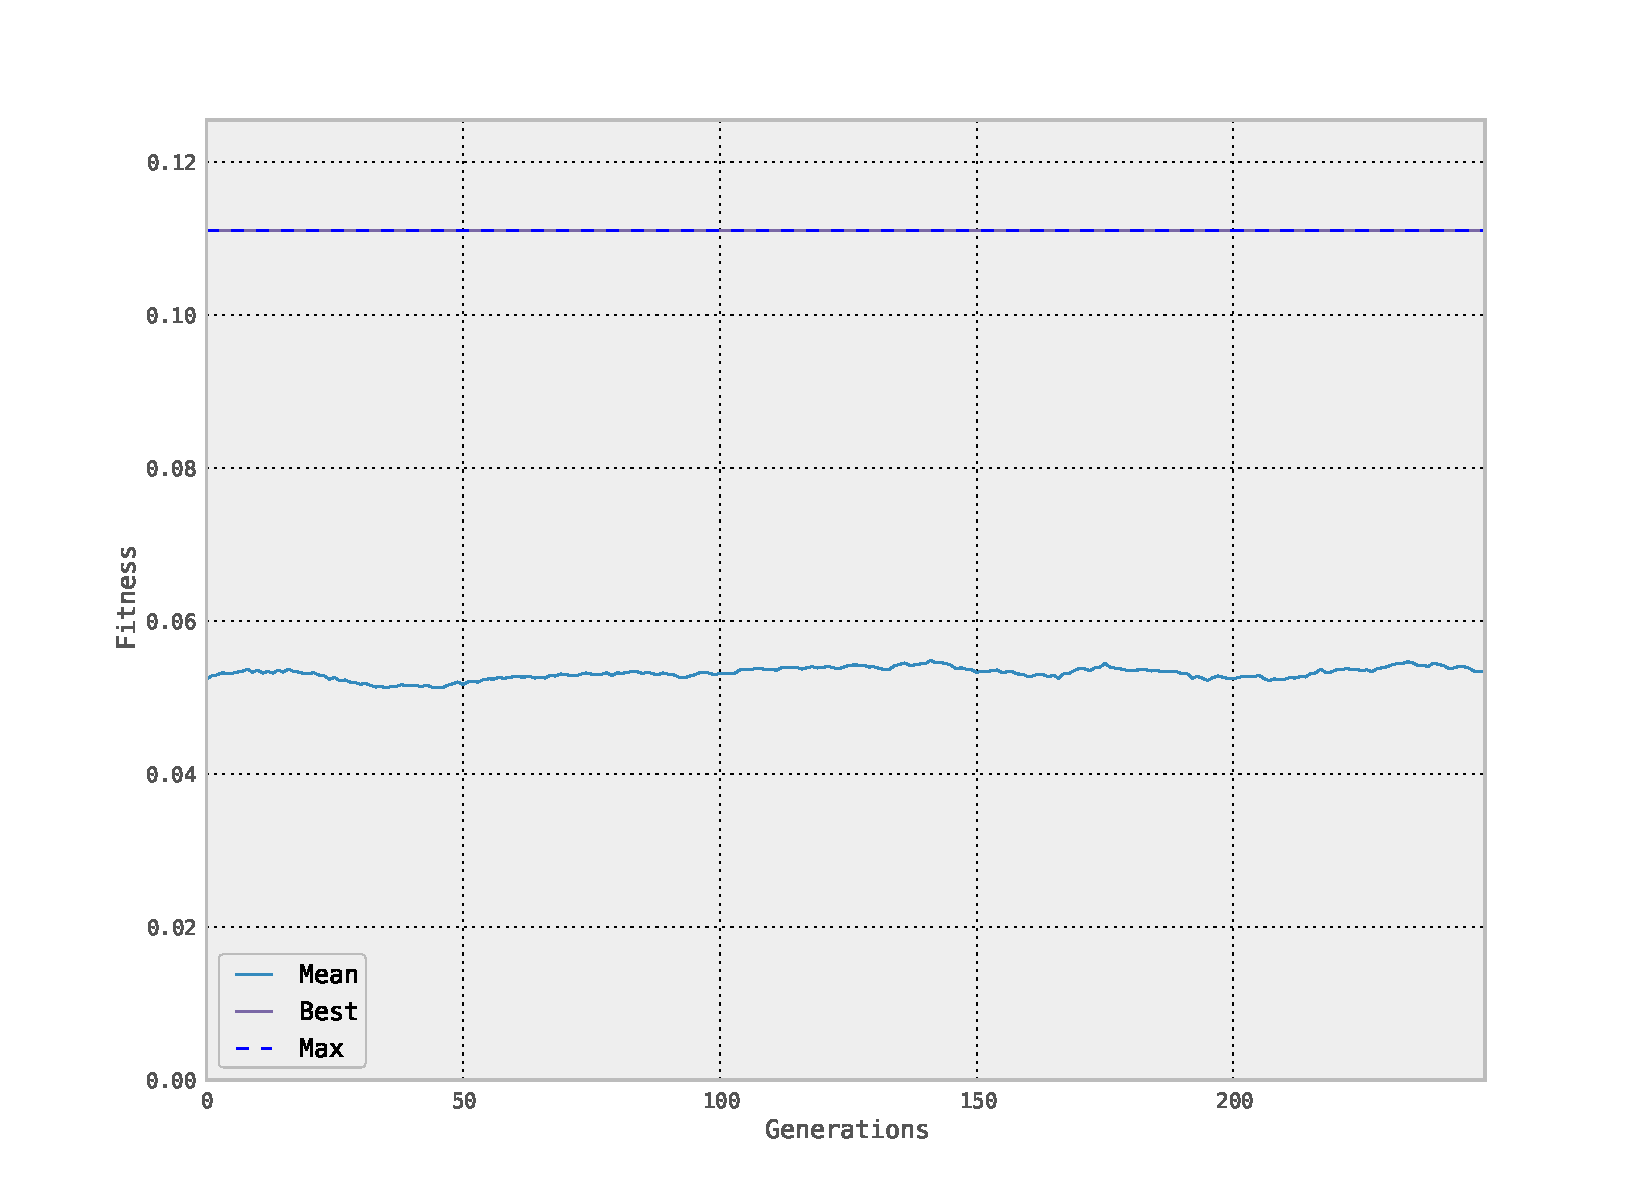
\includegraphics[scale =0.4] {images/section3/fitness_1_100_001.pdf}
	\label{fig:figure51}
}
\subfigure[Pheromones per edge]{
	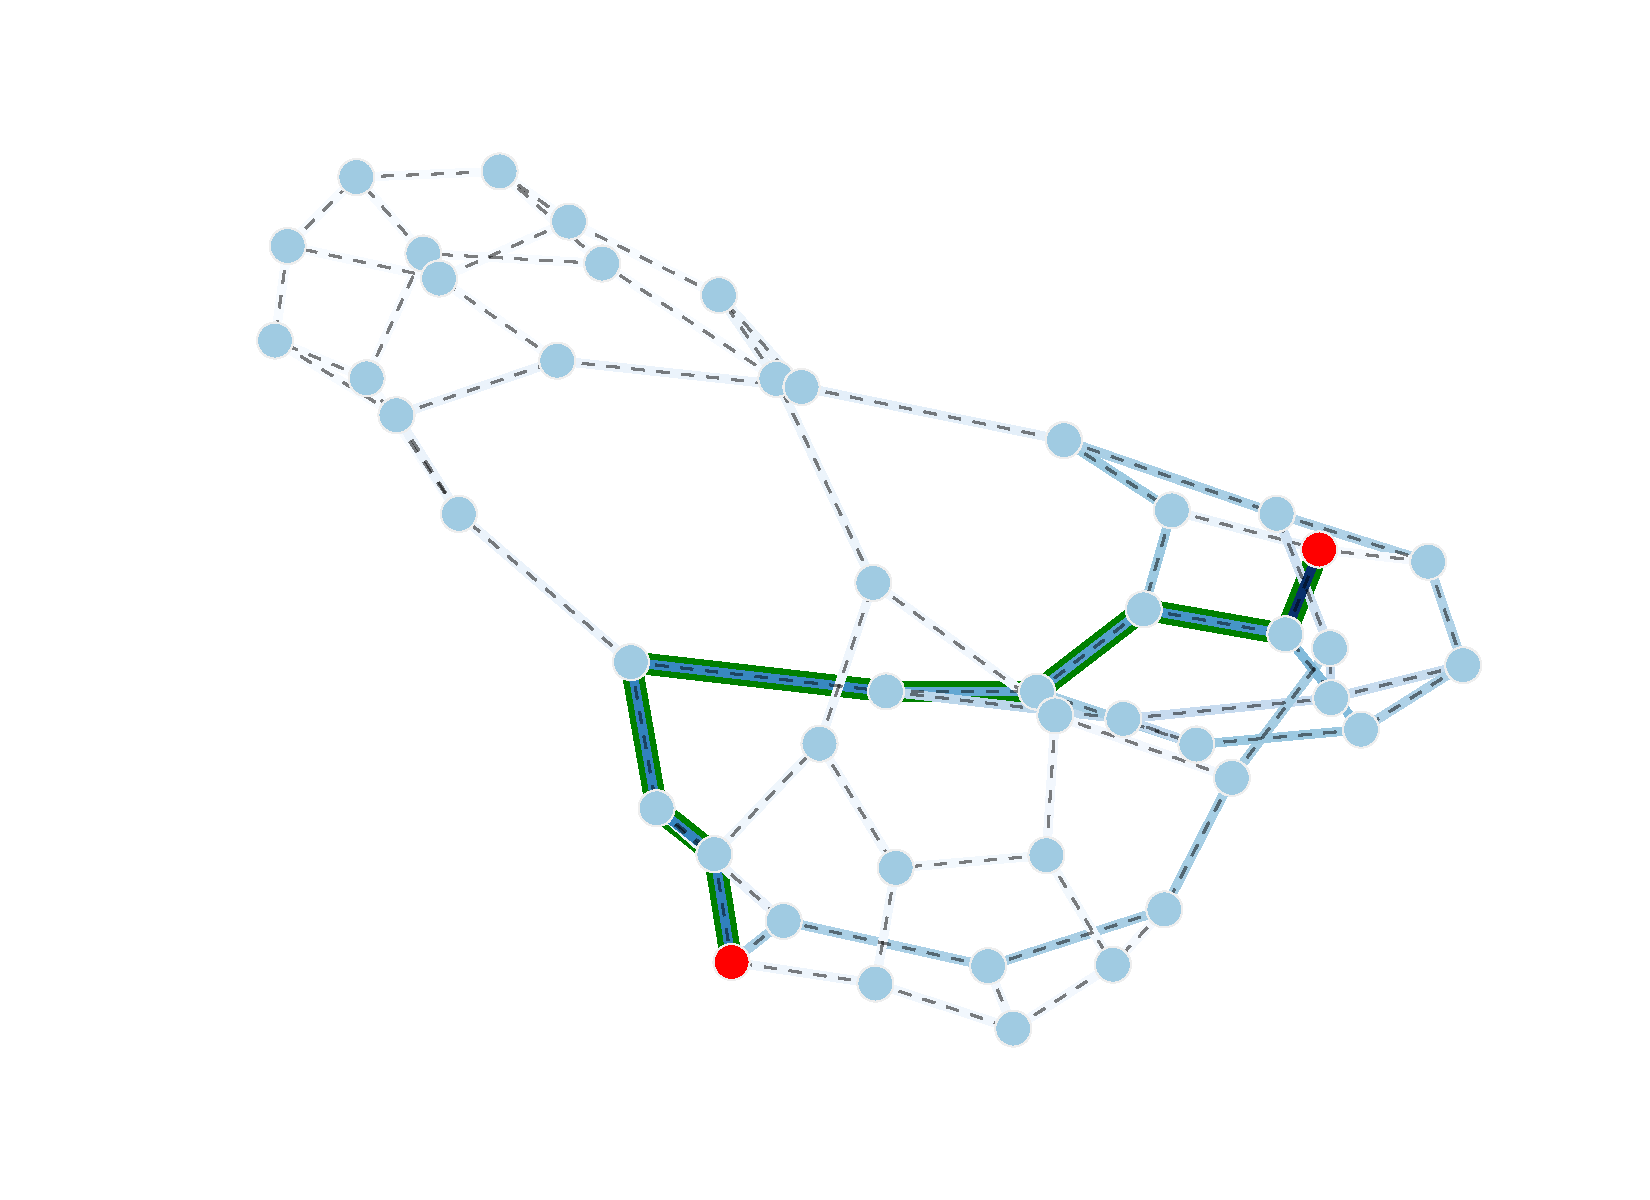
\includegraphics[scale =0.4] {images/section3/pheromones_100_001.pdf}
	\label{fig:figure52}
}
%\caption[Optional caption for list of figures]{Caption of subfigures \subref{fig:subfig1}, \subref{fig:subfig2}}
\label{fig:figure5}
\end{figure}





\newpage
\subsection{Set $\rho = 0.5, k=5$}

\begin{figure}[ht]
\centering
\subfigure[Fitness evolution]{
	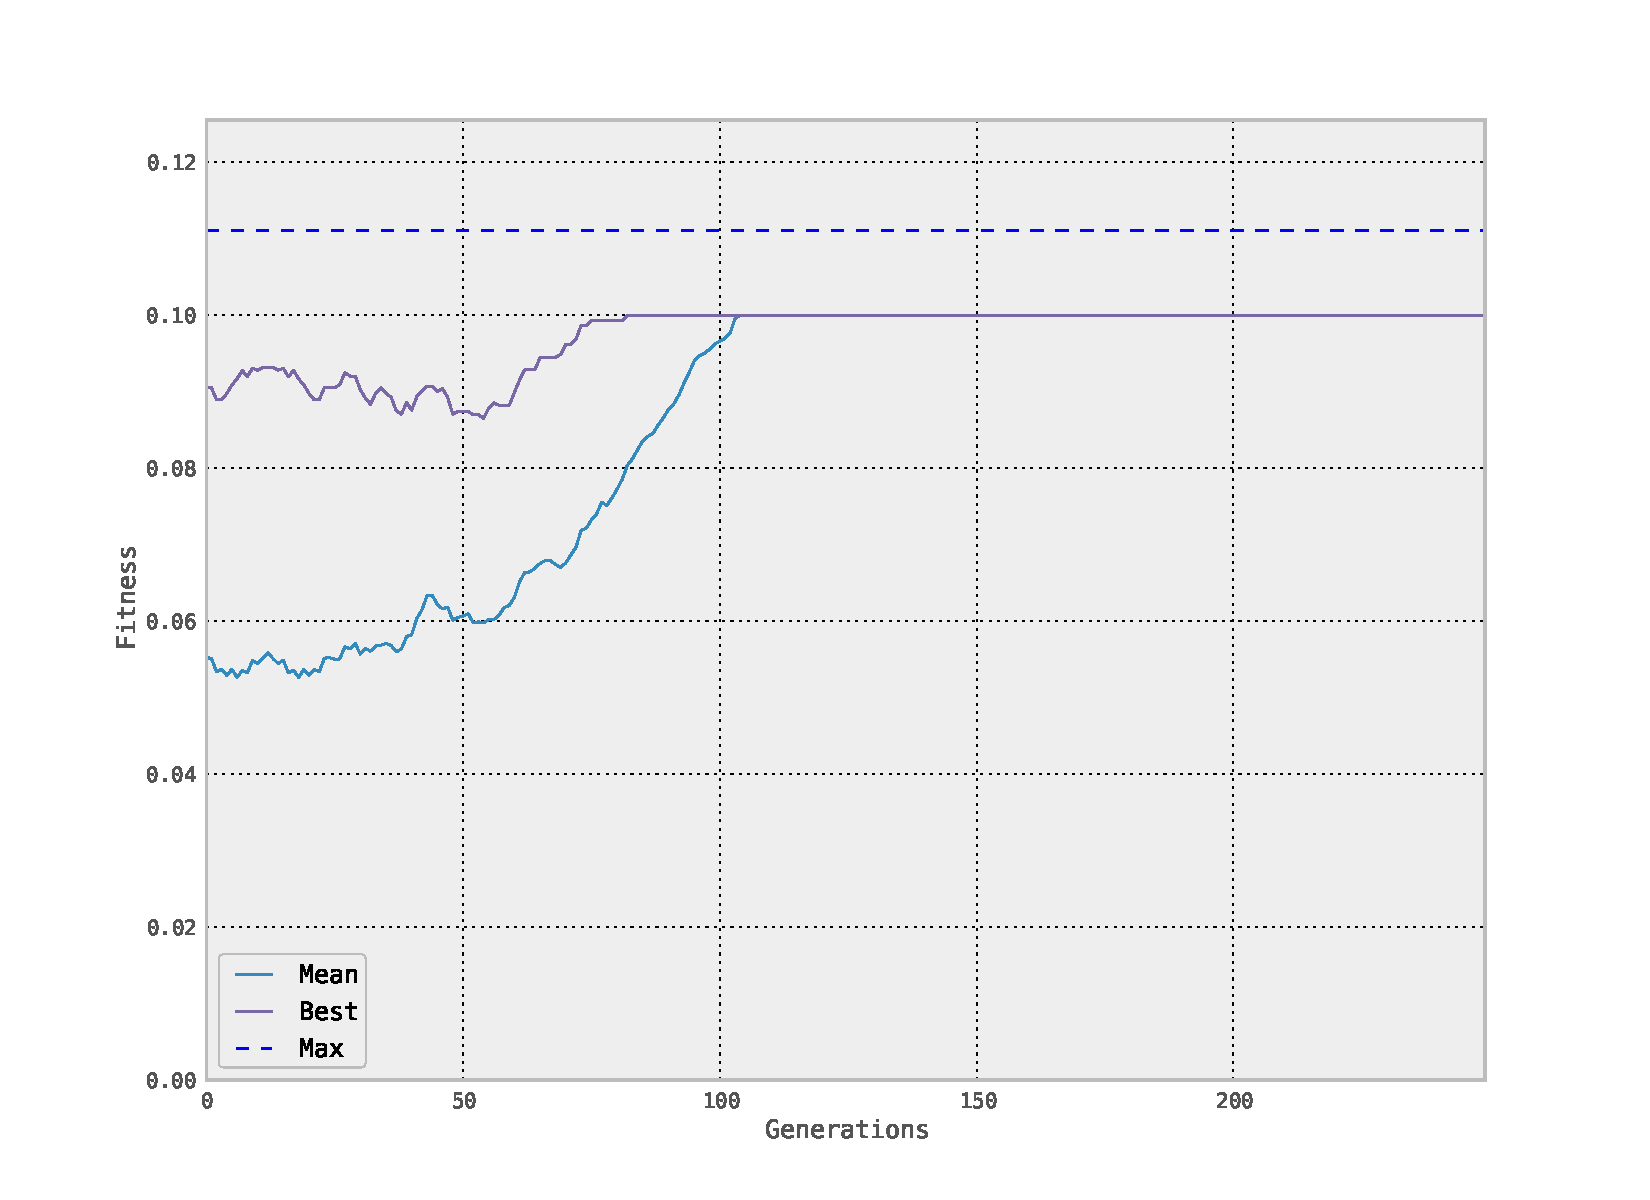
\includegraphics[scale =0.4] {images/section3/fitness_1_5_05.pdf}
	\label{fig:figure61}
}
\subfigure[Pheromones per edge]{
	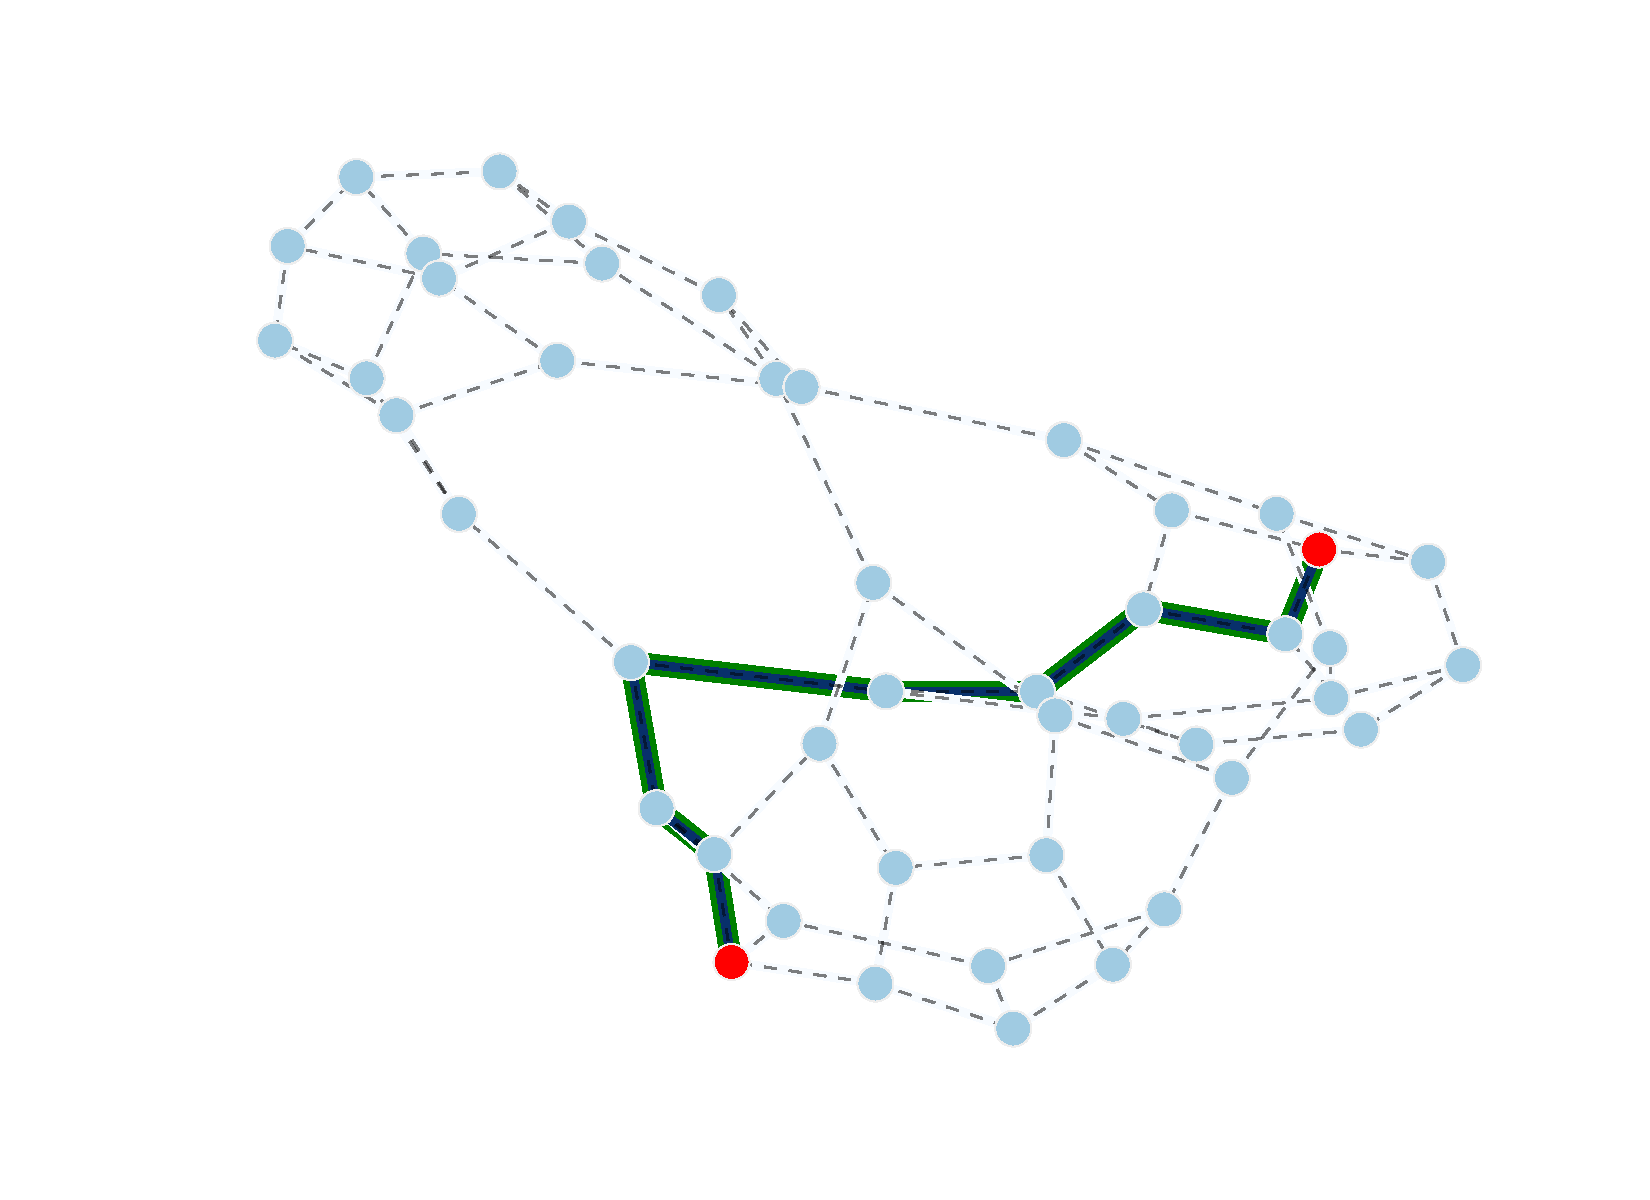
\includegraphics[scale =0.4] {images/section3/pheromones_5_05.pdf}
	\label{fig:figure62}
}
%\caption[Optional caption for list of figures]{Caption of subfigures \subref{fig:subfig1}, \subref{fig:subfig2}}
\label{fig:figure6}
\end{figure}






\newpage
\subsection{Set $\rho = 0.5, k=10$}

\begin{figure}[ht]
\centering
\subfigure[Fitness evolution]{
	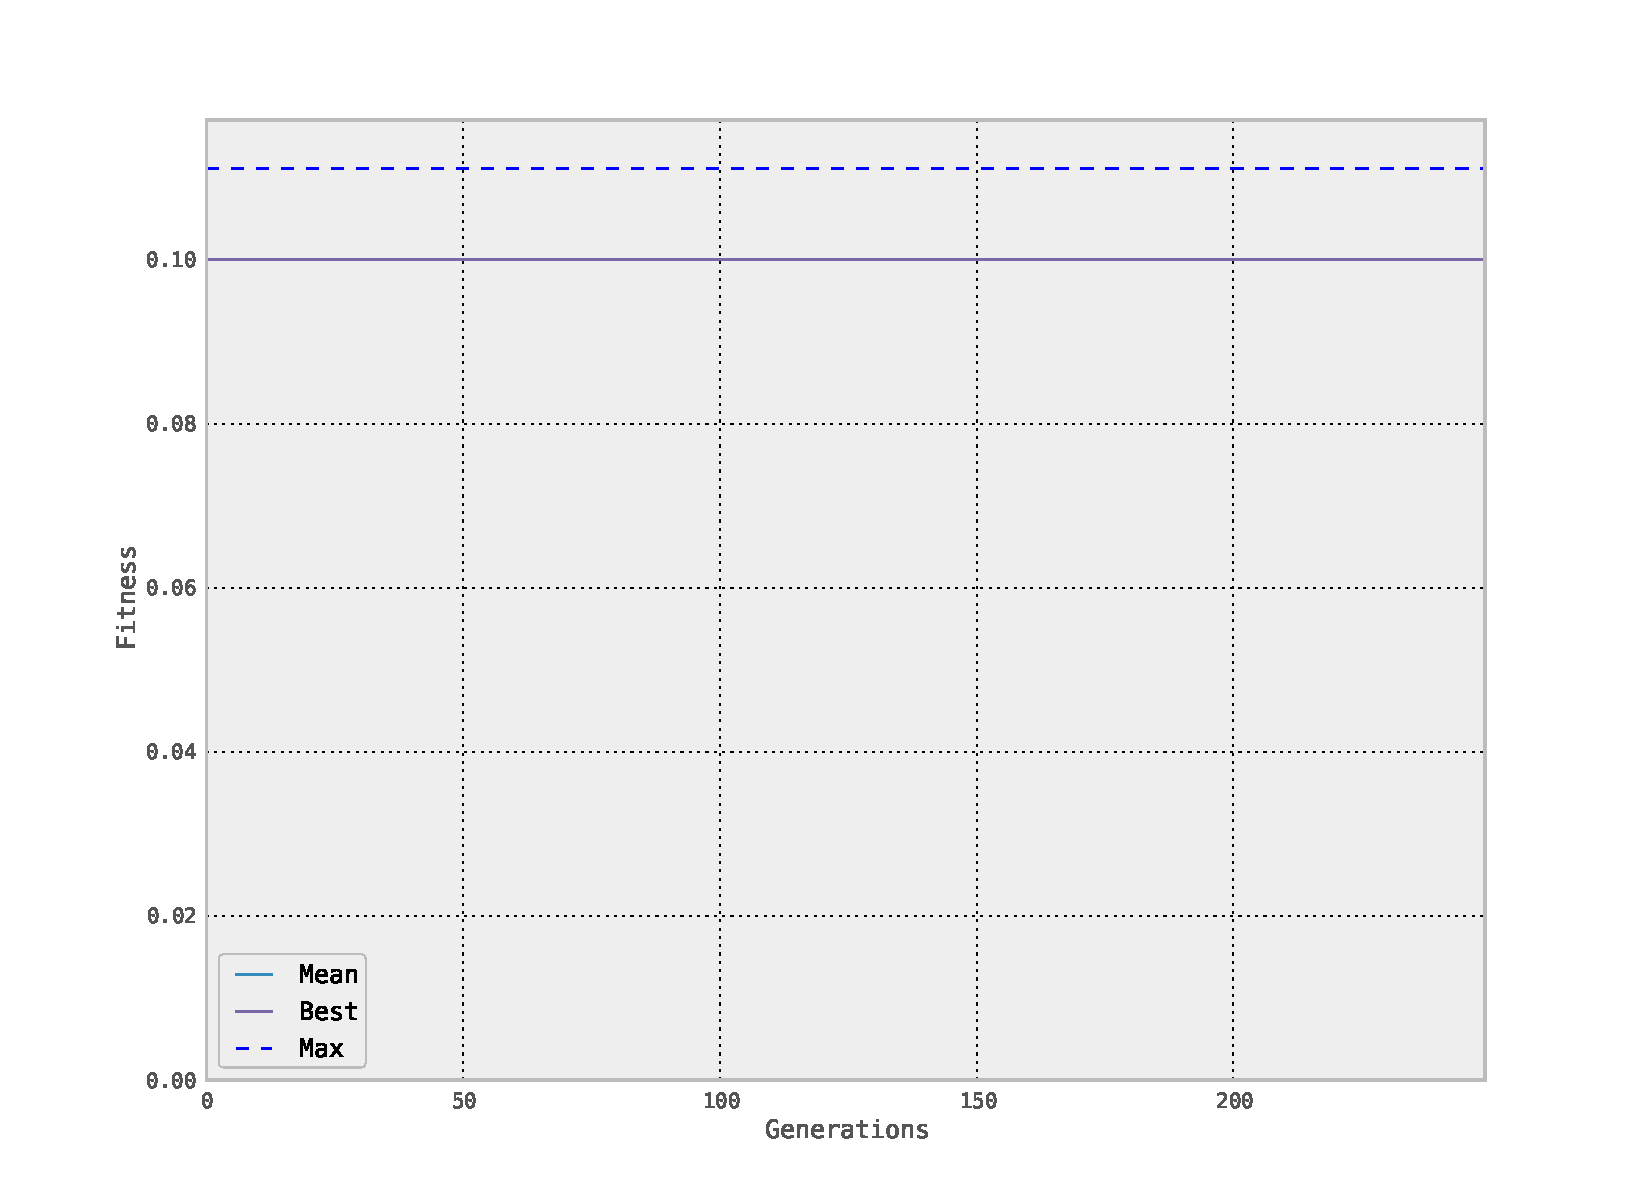
\includegraphics[scale =0.4] {images/section3/fitness_1_10_05.pdf}
	\label{fig:figure71}
}
\subfigure[Pheromones per edge]{
	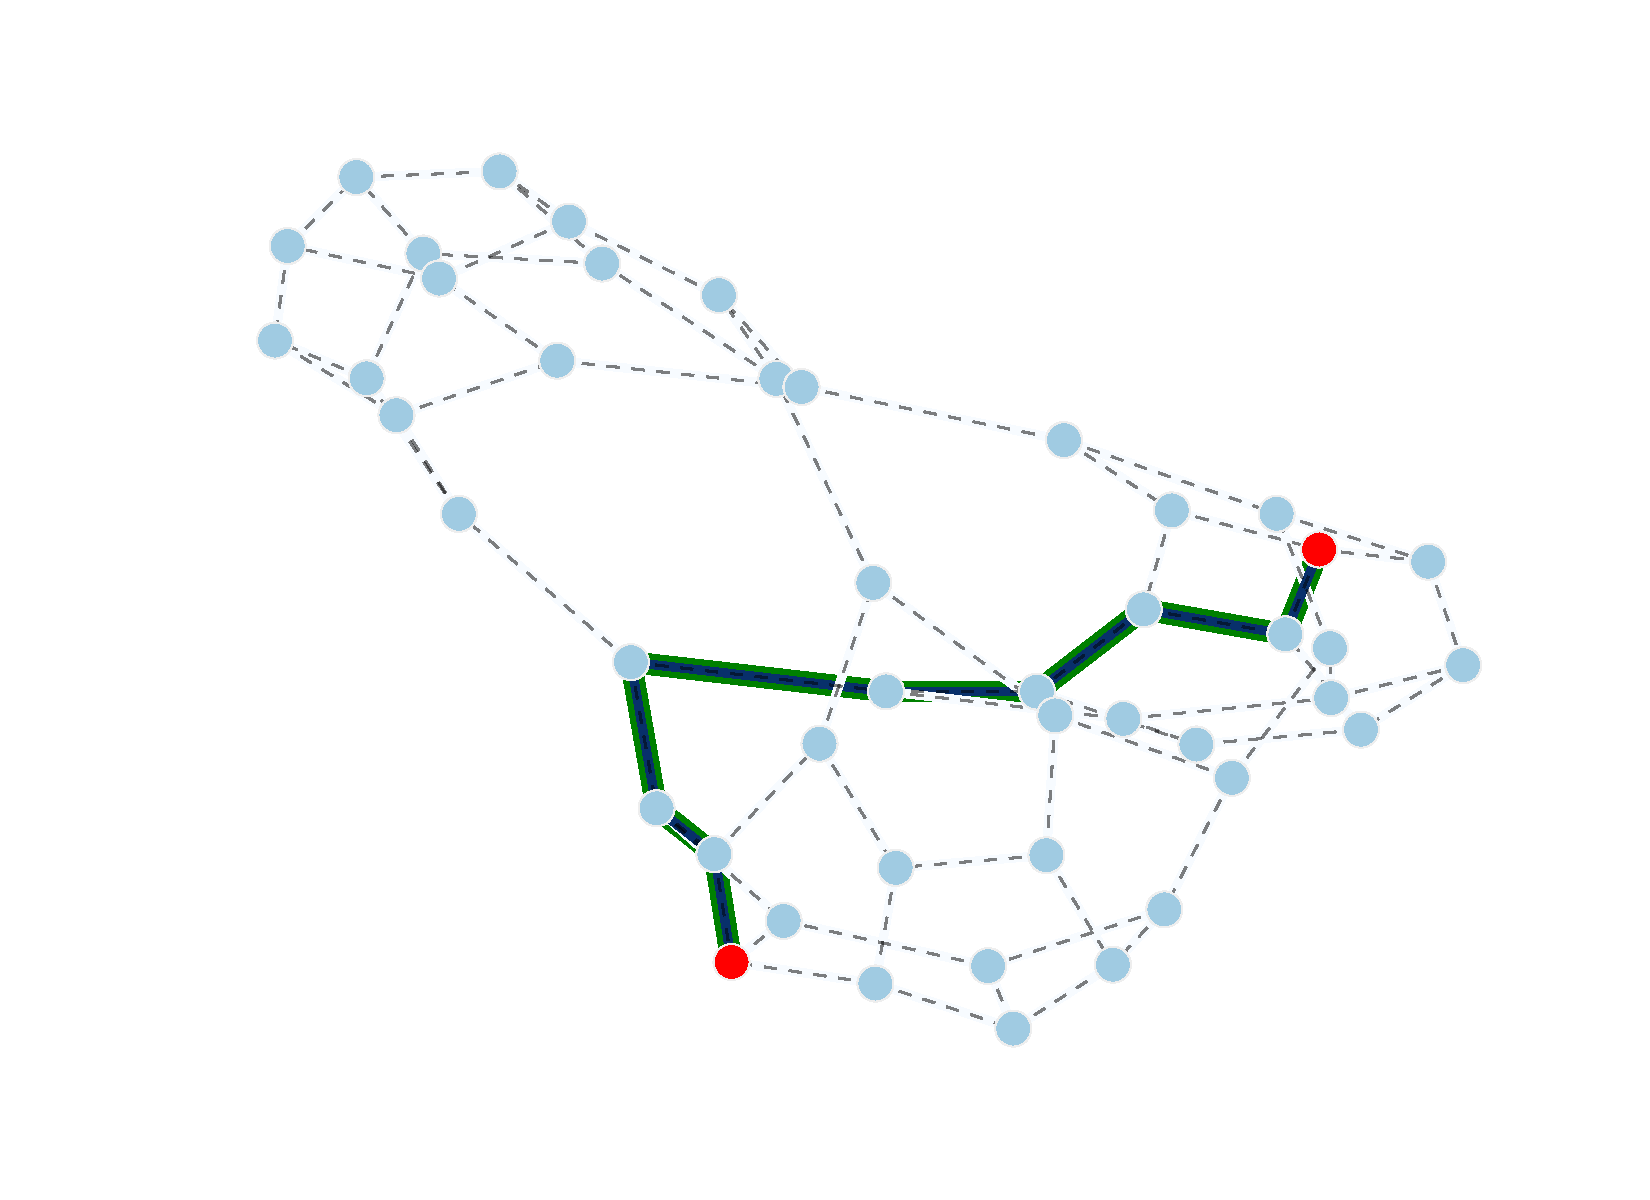
\includegraphics[scale =0.4] {images/section3/pheromones_10_05.pdf}
	\label{fig:figure72}
}
%\caption[Optional caption for list of figures]{Caption of subfigures \subref{fig:subfig1}, \subref{fig:subfig2}}
\label{fig:figure7}
\end{figure}





\newpage
\subsection{Set $\rho = 0.5, k=15$}

\begin{figure}[ht]
\centering
\subfigure[Fitness evolution]{
	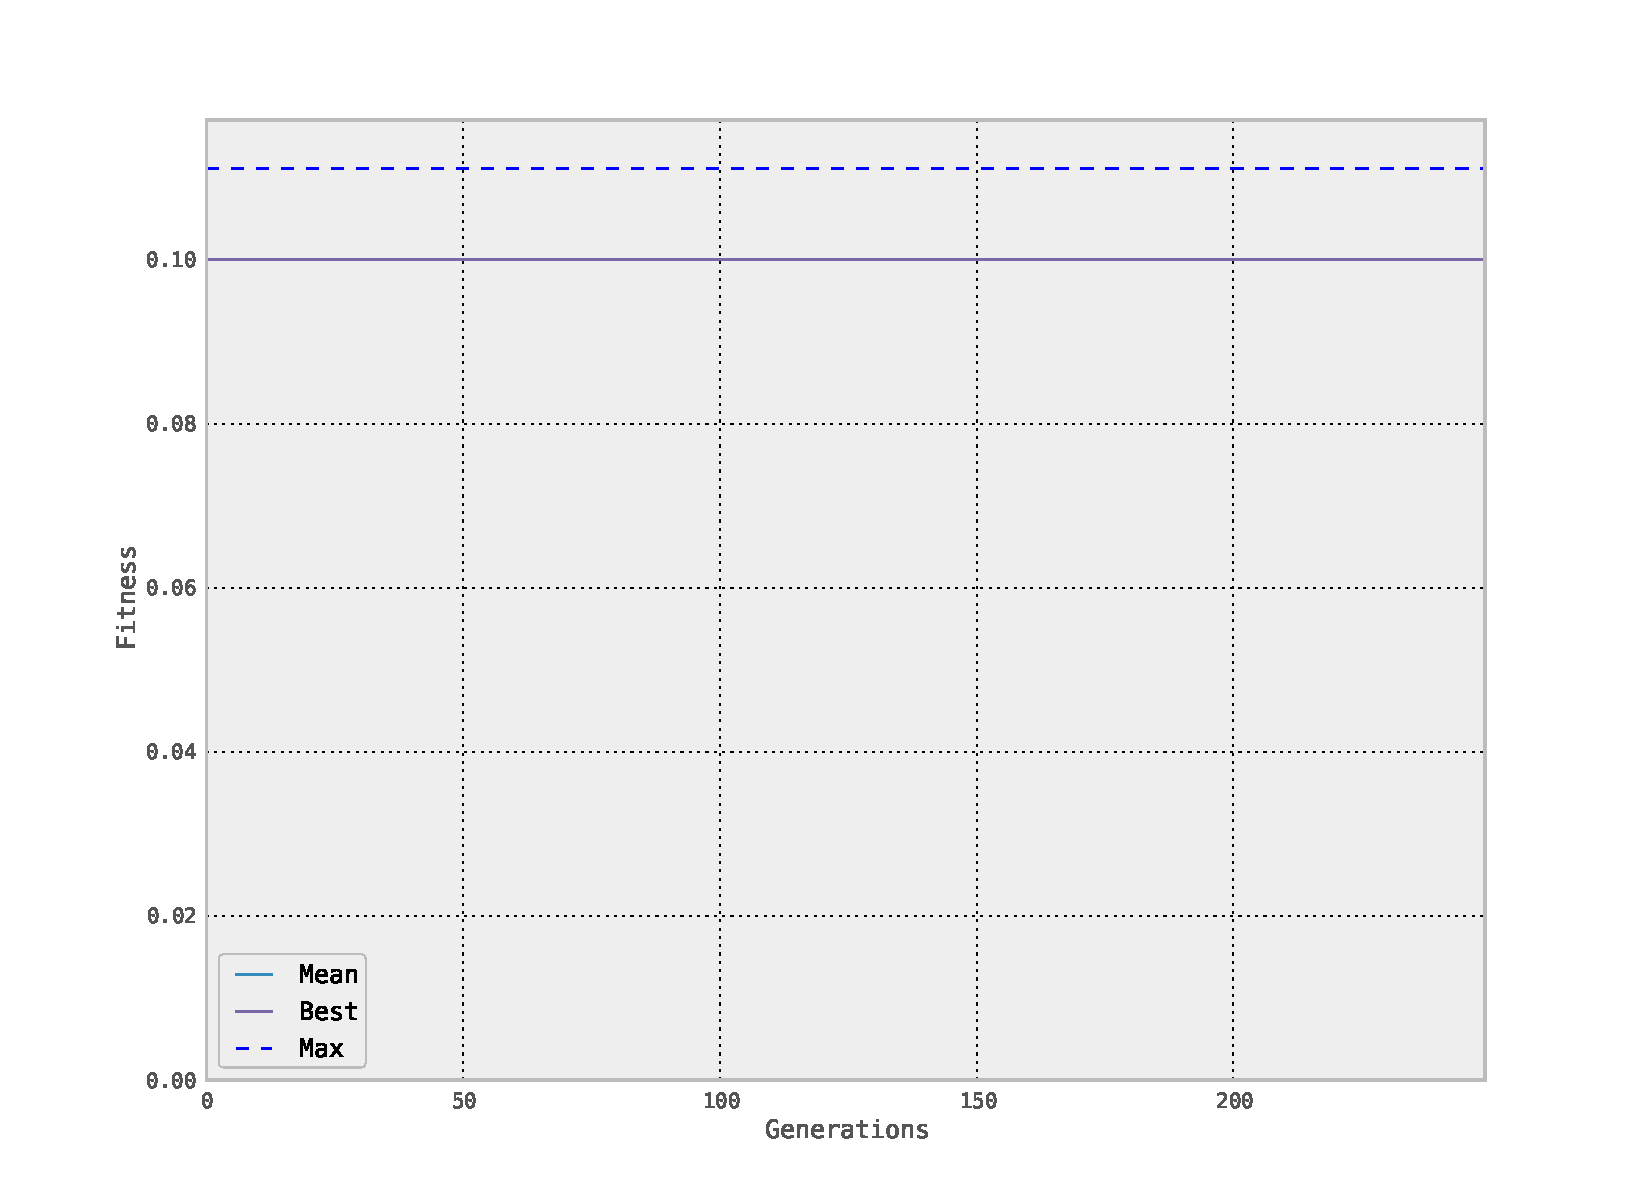
\includegraphics[scale =0.4] {images/section3/fitness_1_15_05.pdf}
	\label{fig:figure81}
}
\subfigure[Pheromones per edge]{
	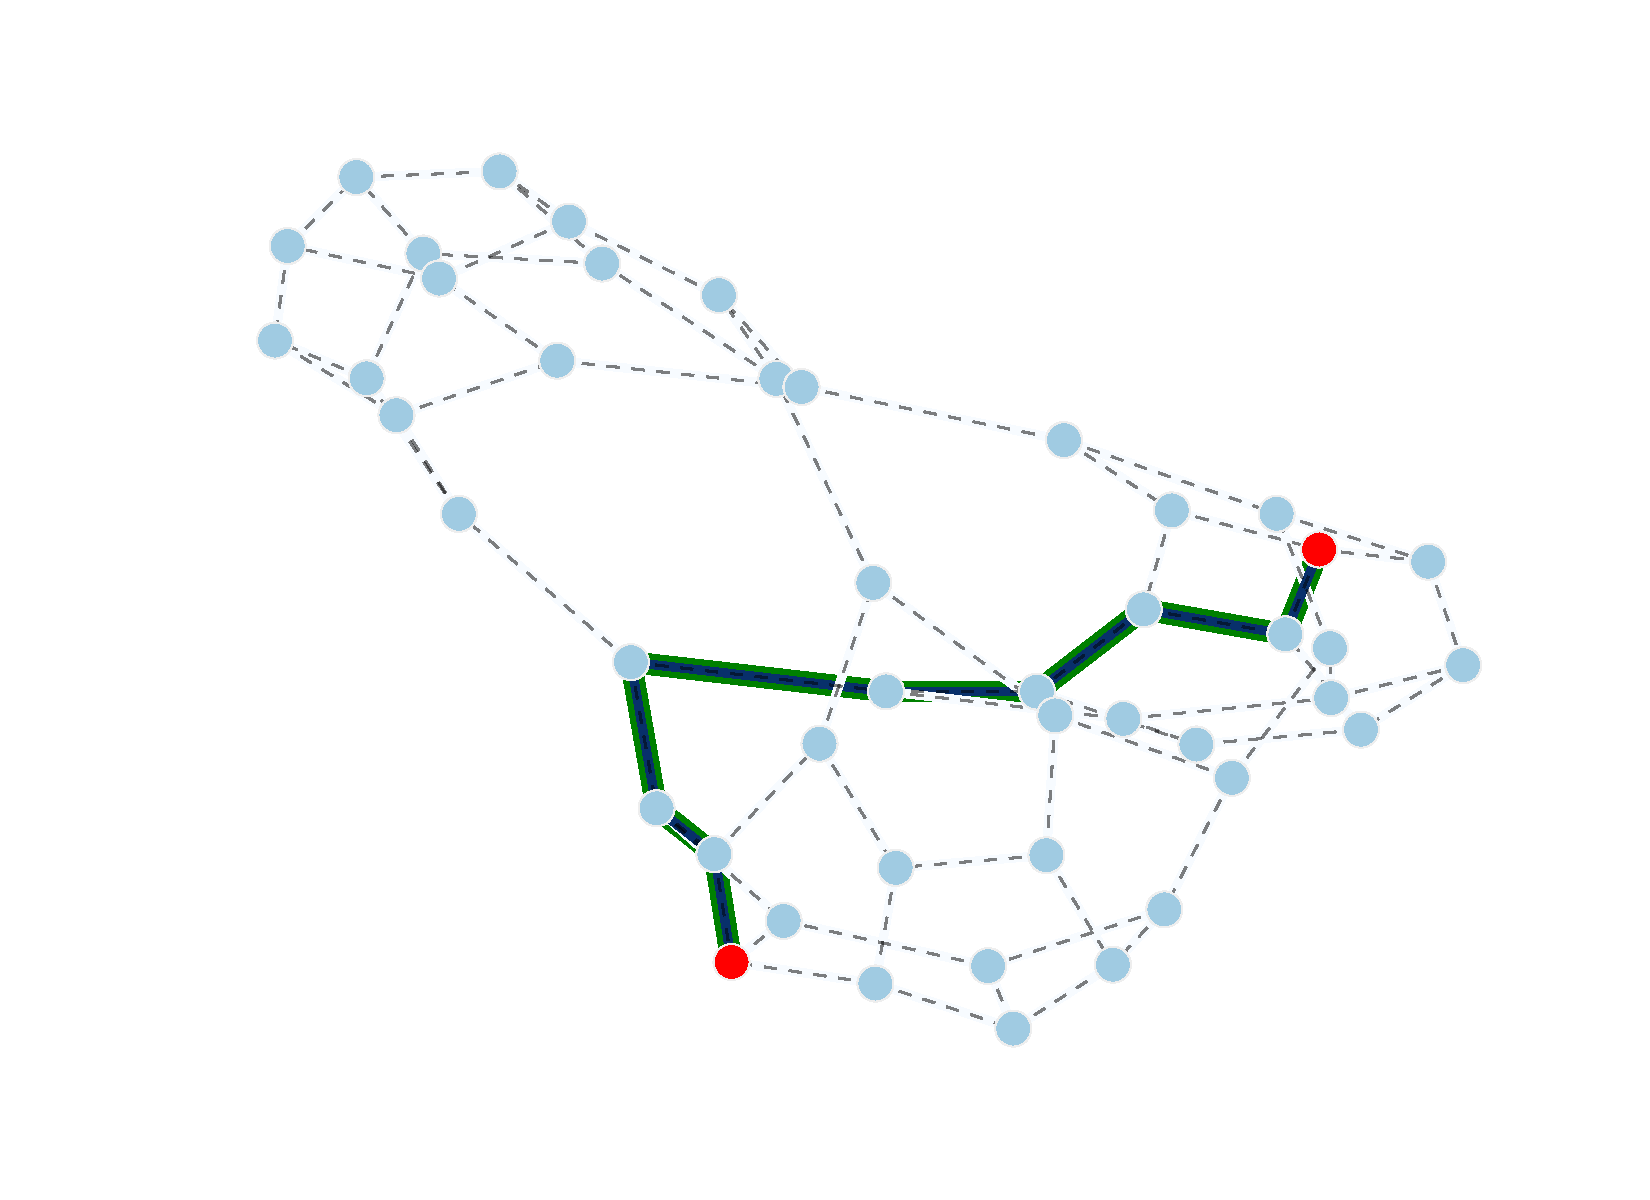
\includegraphics[scale =0.4] {images/section3/pheromones_15_05.pdf}
	\label{fig:figure82}
}
%\caption[Optional caption for list of figures]{Caption of subfigures \subref{fig:subfig1}, \subref{fig:subfig2}}
\label{fig:figure8}
\end{figure}





\newpage
\subsection{Set $\rho = 0.5, k=50$}



\begin{figure}[ht]
\centering
\subfigure[Fitness evolution]{
	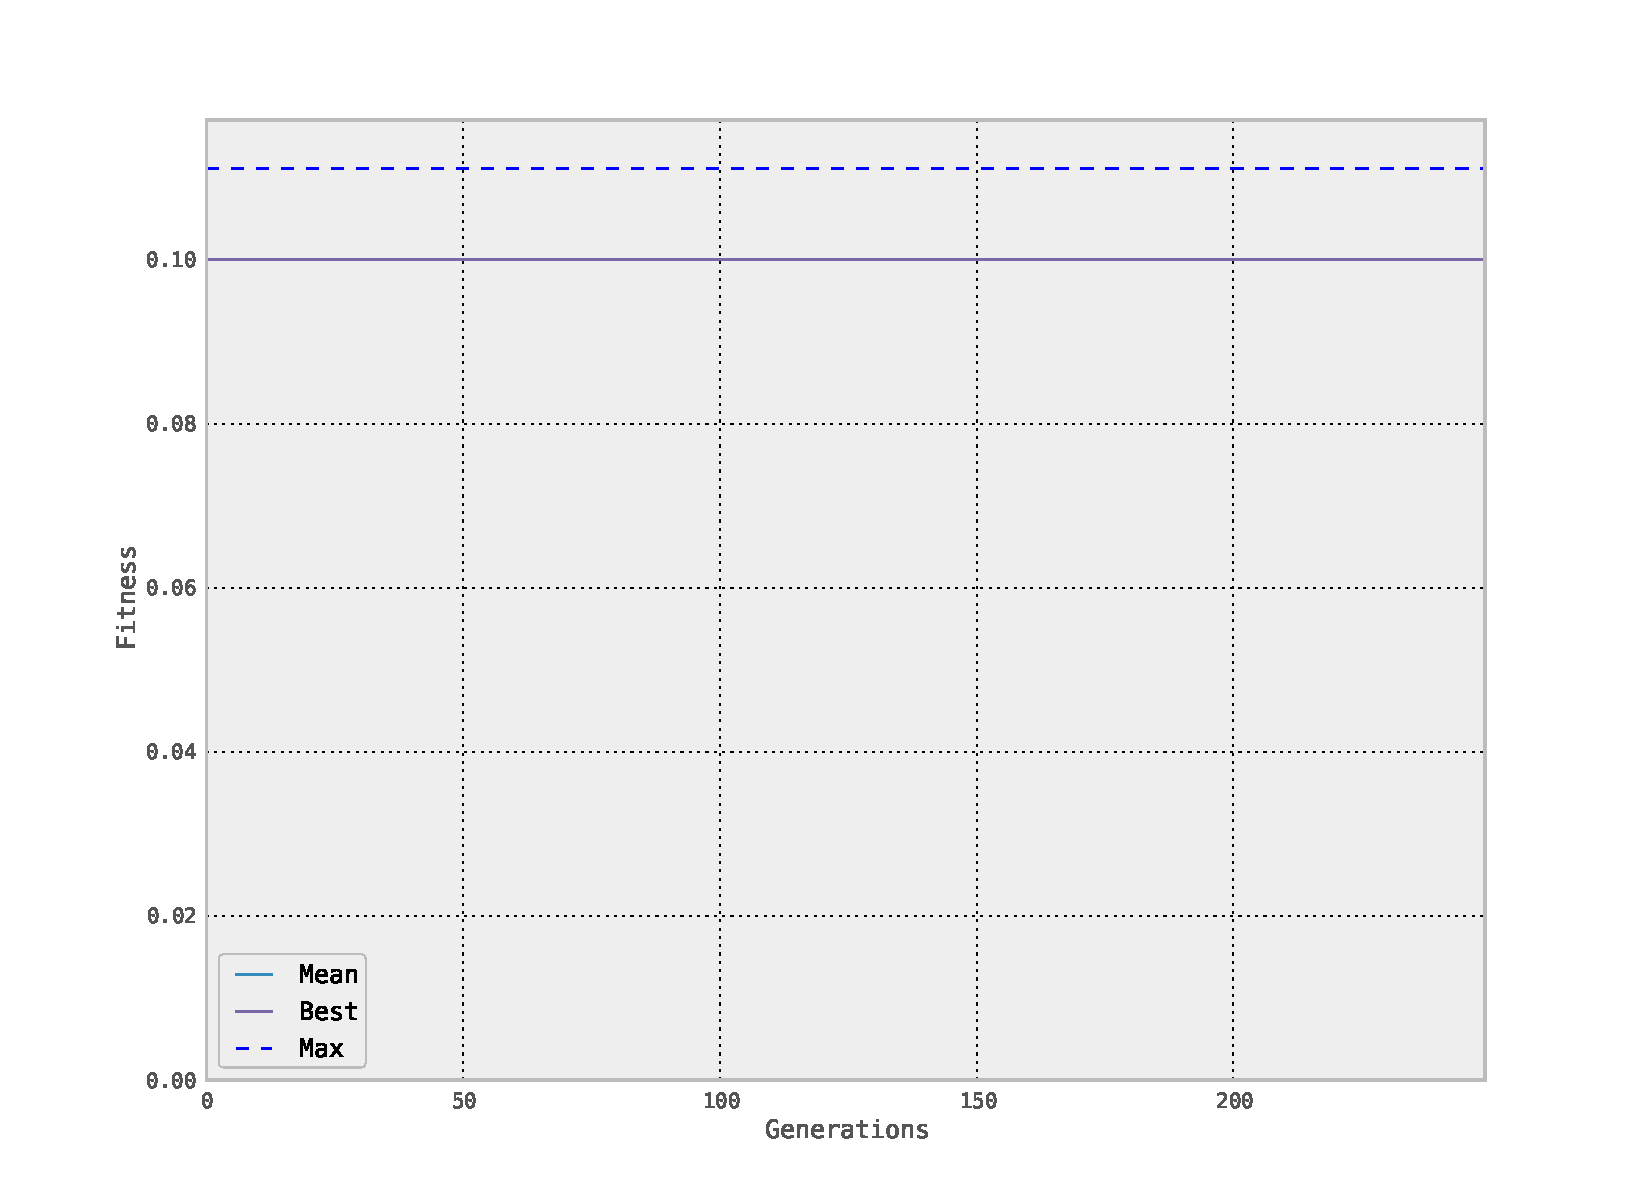
\includegraphics[scale =0.4] {images/section3/fitness_1_50_05.pdf}
	\label{fig:figure91}
}
\subfigure[Pheromones per edge]{
	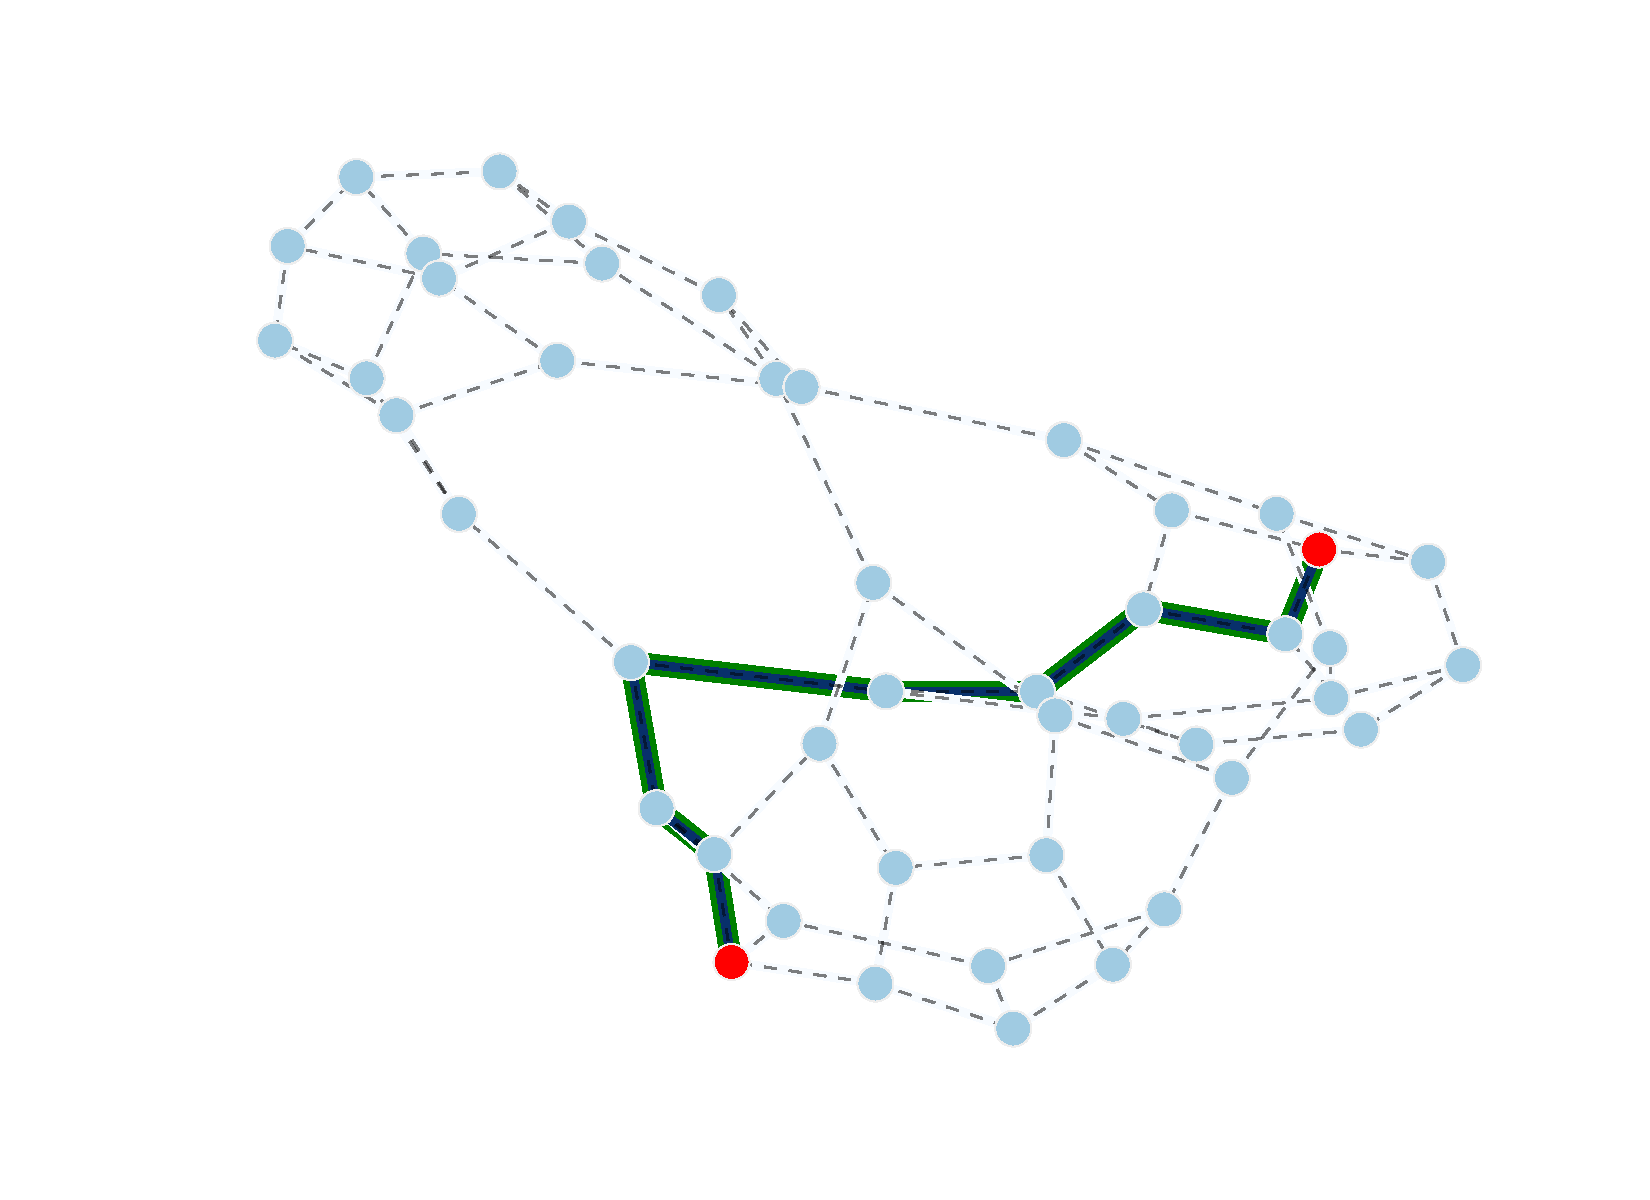
\includegraphics[scale =0.4] {images/section3/pheromones_50_05.pdf}
	\label{fig:figure92}
}
%\caption[Optional caption for list of figures]{Caption of subfigures \subref{fig:subfig1}, \subref{fig:subfig2}}
\label{fig:figure9}
\end{figure}



\newpage
\subsection{Set $\rho = 0.5, k=100$}


\begin{figure}[ht]
\centering
\subfigure[Fitness evolution]{
	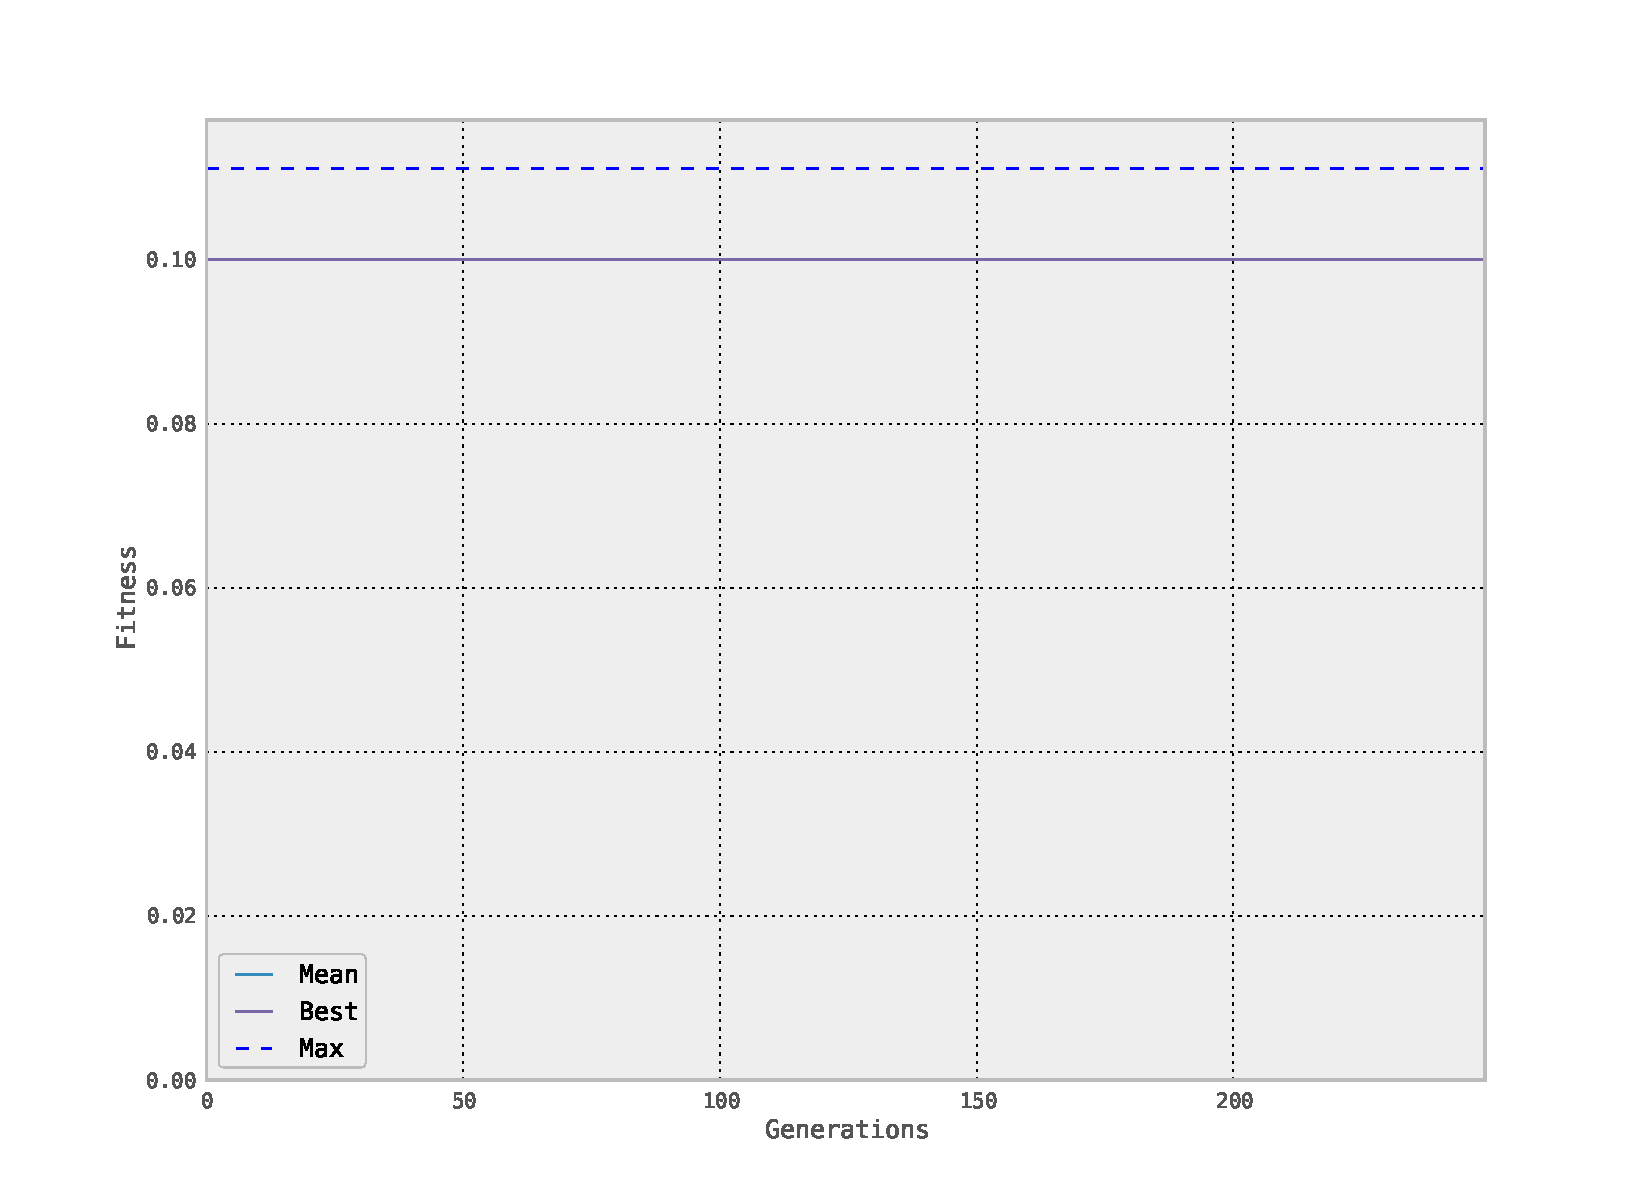
\includegraphics[scale =0.4] {images/section3/fitness_1_100_05.pdf}
	\label{fig:figure101}
}
\subfigure[Pheromones per edge]{
	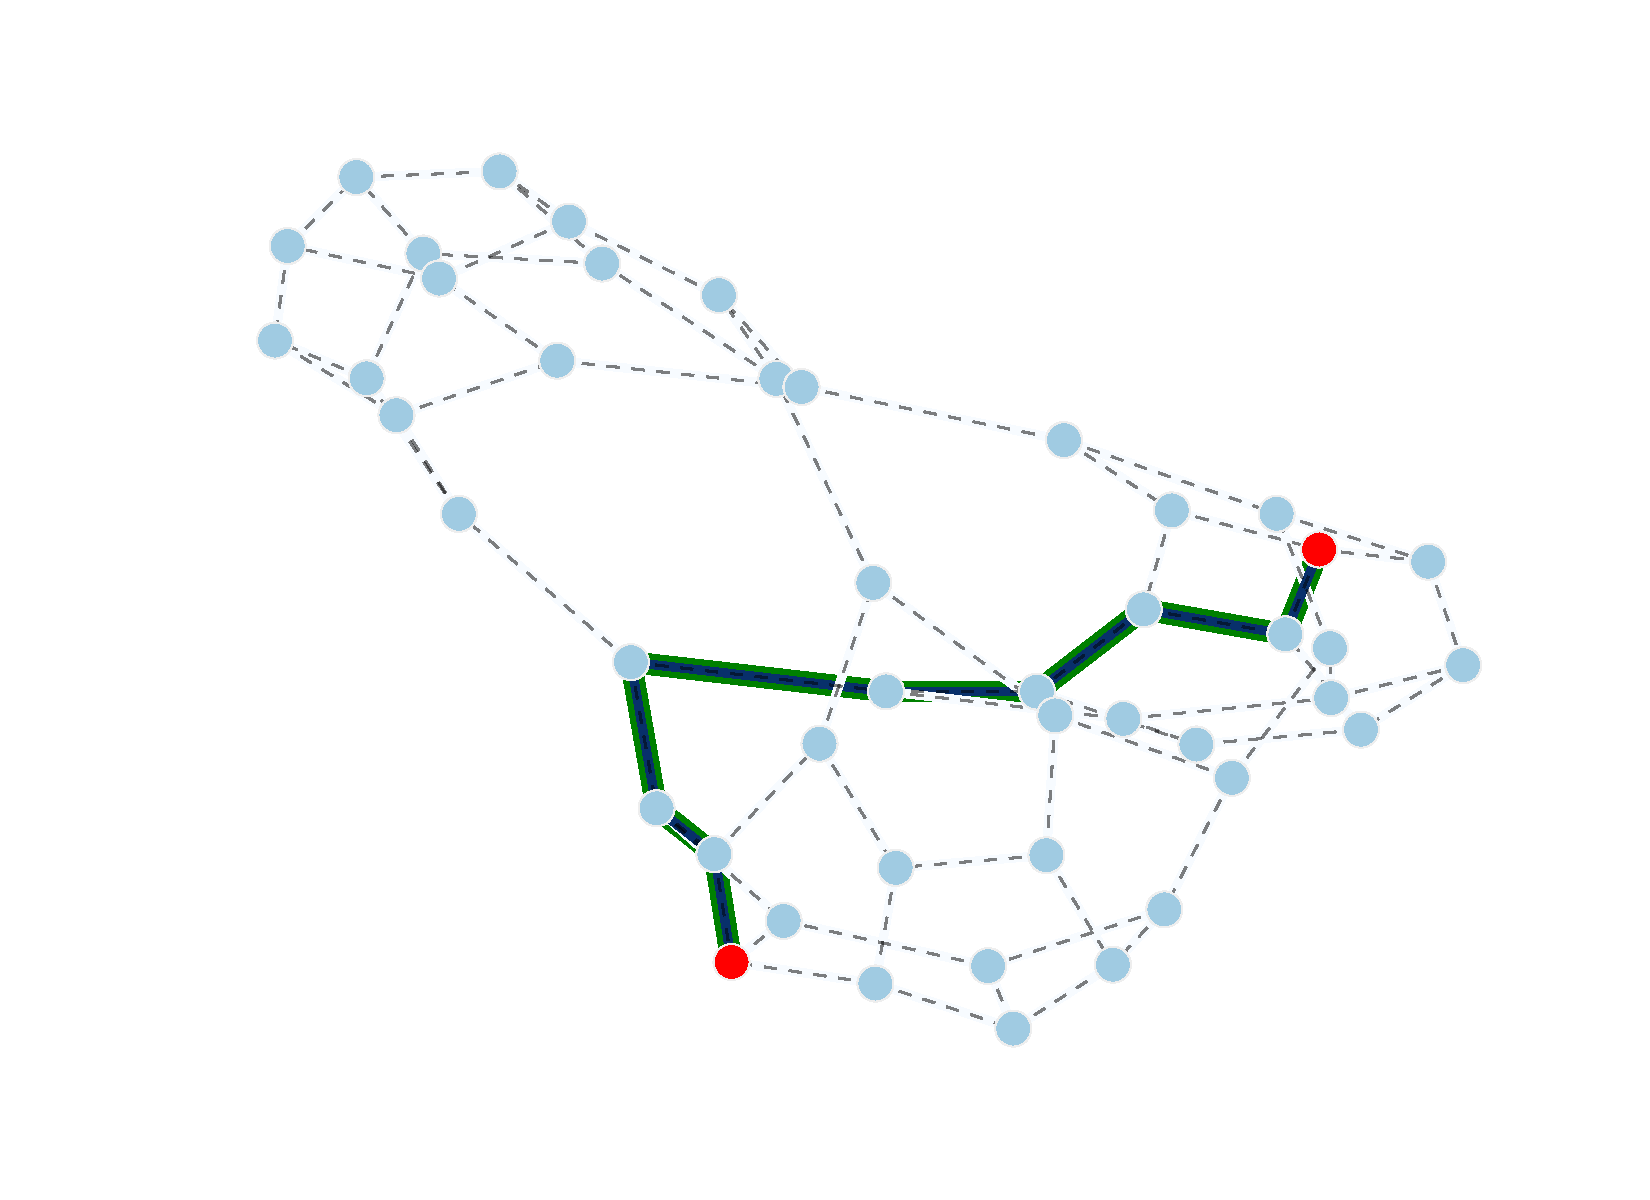
\includegraphics[scale =0.4] {images/section3/pheromones_100_05.pdf}
	\label{fig:figure102}
}
%\caption[Optional caption for list of figures]{Caption of subfigures \subref{fig:subfig1}, \subref{fig:subfig2}}
\label{fig:figure10}
\end{figure}


\newpage
\subsection{Conclusions}
We can conclude that in the first configuration with $\rho = 0.1$ the algorithm are able to remember some paths in order to achieve the best one. The second configuration has a high value to $\rho = 0.5$, therefore, algorithm can discard best solutions growing the exploration factor, however, sometimes can not reach the goal of get the shortest path
\\
\\
We can see that $k=5$ and $k=10$ is not enought to reach the best fitness and therefore to reach the shortest path.